Die Systemtheorie beschreibt Systeme unter anderem durch den Zusammenhang von Signalen am Systemeingang und - Ausgang. Dabei k\"{o}nnen Signale und Systeme von unterschiedlichster Natur sein. Ein System ist zum Beispiel ein elektrisches Netzwerk, das durch Eingangs- und Ausgangsspannung beschrieben werden kann. Ein weiteres System ist ein Regler, der den F\"{u}llstand eines Beh\"{a}lters regelt. Er besitzt ein elektrisches Eingangssignal, dass die F\"{u}llstandsh\"{o}he repr\"{a}sentiert. Mit seinem Ausgangssignal wird ein Stellwerk angesteuert, das den Zufluss in den Beh\"{a}lter steuert.

\noindent Signale k\"{o}nnen \"{u}ber unterschiedliche Merkmale klassifiziert werden. Aus der Einteilung in zeitkontinuierliche Signale (Teil A), zeitdiskrete Signale (Teil B) und stochastische Signale (Teil C) ergibt sich die Struktur dieser Buchreihe. Dar\"{u}ber hinaus werden andere Klassifizierungsmerkmale vorgestellt.

\noindent F\"{u}r die Charakterisierung von Systemen werden Testfunktionen eingesetzt werden, die eine besonders anschauliche Interpretation des Ausgangssignals erm\"{o}glichen. Dazu geh\"{o}ren Sprungfunktionen, Rampenfunktionen und Impulsfunktionen. Diese Funktionen werden diskutiert und das Rechnen mit diesen Testfunktionen an Beispielen erl\"{a}utert. In einem Experiment am Ende des Kapitels wird der Begriff der Impulsfunktion verdeutlicht.

\noindent Sogenannte lineare, zeitinvariante Systeme zeichnen sich dadurch aus, dass f\"{u}r sie das sogenannte Superpositionsprinzip gilt. Kann ein Eingangssignal aus einer Linearkombination bekannter Signale beschrieben werden, ergibt sich das Ausgangssignal aus derselben Linearkombination der zugeh\"{o}rigen Ausgangssignale. Deshalb wird die Signalalgebra vorgestellt, die die Zerlegung von Signalen in elementare Signale erm\"{o}glicht.

\noindent Das Ausgangsignal oder die Reaktion eines Systems kann vielfach \"{u}ber Kosinus- und Exponentialfunktionen beschrieben werden. Beide Funktionen k\"{o}nnen zu komplexen Exponentialfunktionen zusammengefasst werden. Komplexe Exponentialfunktionen werden dazu verwendet, das Einschwingverhalten von Systemen effizient zu beschreiben. Das Rechnen mit komplexen Exponentialfunktionen wird eingef\"{u}hrt und ge\"{u}bt.

\noindent Werden physikalische Gr\"{o}{\ss}en auf Einheiten und typische Gr\"{o}{\ss}enordnungen bezogen, ergeben sich \"{u}bersichtlichere Zahlenwerte und vereinfachte Darstellungen. Im letzten Teil des Kapitels wird gezeigt, wie Signale normiert werden. 


\subsection{ Klassen von Signalen}


\subsubsection{ Kontinuierliche und diskrete Signale}
Signale lassen sich zun\"{a}chst hinsichtlich ihres Verlaufes in kontinuierliche und diskrete Signale einteilen. So ist zum Beispiel der Spannungsverlauf an einem Mikrofon ein zeitkontinuierliches Signal, das zu jedem beliebigen Zeitpunkt t definiert ist. Sein Wertevorrat ist ebenfalls kontinuierlich, sodass von einem zeitkontinuierlichen und wertkontinuierlichen Signal gesprochen wird.

\noindent Wird dieselbe analoge Spannung mit einem Analog-Digital-Wandler digitalisiert, so wird das Signal zu definierten Zeitpunkten einer endlichen Anzahl von Quantisierungsstufen zugeordnet. Das Signal wird also in zweierlei Hinsicht diskretisiert. Nach der Digitalisierung liegt ein zeit- und wertdiskretes Signal vor.

\noindent Ein Beispiel f\"{u}r ein zeitdiskretes und wertkontinuierliches Signal ist die Messung einer wertkontinuierlichen Gr\"{o}{\ss}e, die jeden Tag zu einer bestimmten Uhrzeit durchgef\"{u}hrt wird. Die Messgr\"{o}{\ss}e ist kontinuierlich, aber sie ist zwischen den einzelnen Messzeitpunkten nicht bekannt.

\noindent Ein wertediskretes und zeitkontinuierliches Signal ist zum Beispiel der Lagerbestand eines Bauteils. Es k\"{o}nnen nur ganze Bauelemente dem Lager entnommen werden, sodass der Lagerbestand wertediskret ist. Es ist aber zu jedem Zeitpunkt bekannt, wie viele Bauelemente eines bestimmten Typs vorhanden sind. Das Signal ist zeitkontinuierlich.\newline

\noindent Bild \ref{fig:DiskreKontinuerlich} stellt ein Signal in allen m\"{o}glichen Kombinationen der Diskretisierung in Zeit und Wertevorrat an einem Signal dar. 

\clearpage
\begin{figure}[H]
  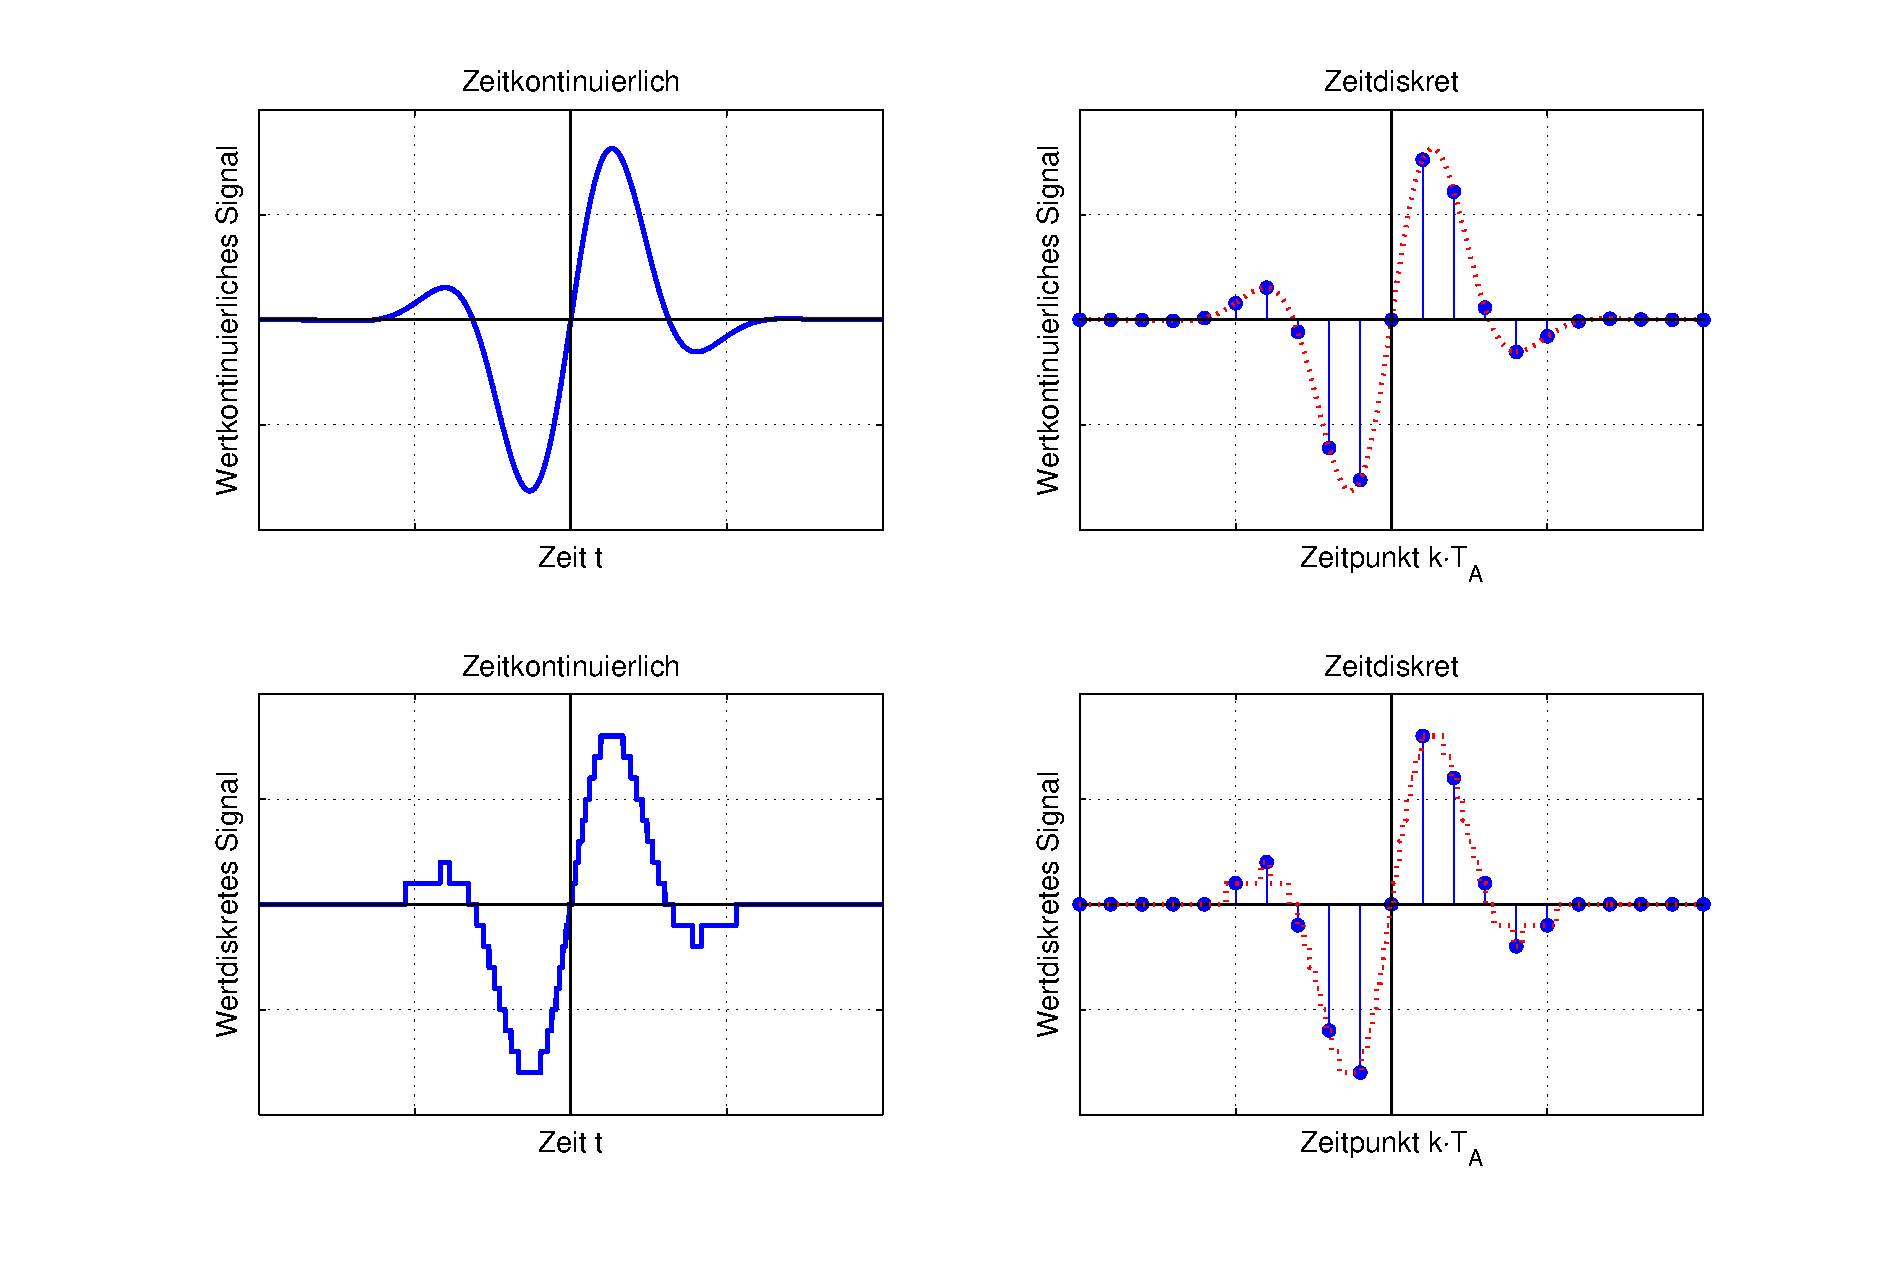
\includegraphics[width=1.0\textwidth]{Kapitel1/Bilder/image1.eps}
  \caption{Darstellung wertkontinuierlicher und wertdiskreter Signale in zeitkontinuierlicher und zeitdiskreter Form}
  \label{fig:DiskreKontinuerlich}
\end{figure}

\noindent In den folgenden Kapiteln beschränken sich die Darstellungen auf werte- und zeitkontinuierliche Signale. Der Übergang zu diskreten Signalen erfolgt mit dem Abtasttheorem im Teil B dieser Buchreihe.


\subsubsection{ Determinierte und zuf\"{a}llige Signale}
Determinierte Signale lassen sich durch eine mathematische Vorschrift in ihrem zeitlichen Verlauf angeben. Sie k\"{o}nnen implizit oder explizit definiert sein. Bei einem explizit definierten Signal l\"{a}sst sich der zu einem Zeitpunkt t geh\"{o}rende Wert direkt ablesen. Ein Beispiel daf\"{u}r ist eine abklingende Sinusfunktion.

\begin{equation}\label{eq:oneone}
x(t)=10\cdot e^{\displaystyle -a\cdot t^{2}} \cdot\sin (b\cdot t)
\end{equation}

\noindent Bei der impliziten Definition eines Signals ist der Signalwert zwar eindeutig bestimmt, er muss aber zun\"{a}chst durch weitere Umformungen bestimmt werden. Ein Beispiel f\"{u}r ein implizit definiertes Signal ist eine Differentialgleichung.

\begin{equation}\label{eq:onetwo}
\dfrac{dx}{dt} +3\cdot \dfrac{d^{2} x}{dt^{2} } =5\cdot x(t)+\sin (\omega \cdot t)
\end{equation}

\noindent mit der Anfangsbedingung y(t = 0) = y${}_{0}$. Unabh\"{a}ngig von der Art der Definition ist der Wert eines determinierten Signals zu jedem Zeitpunkt exakt definiert.

\noindent Zuf\"{a}llige Signale k\"{o}nnen nicht exakt angegeben werden, f\"{u}r sie sind lediglich statistische Eigenschaften bekannt. Beispiele f\"{u}r zuf\"{a}llige Signale sind Rauschsignale, Fernsehsignale oder Sprachsignale. Information, die \"{u}bertragen werden soll, ist zuf\"{a}llig. W\"{a}re das Signal bekannt, m\"{u}sste es nicht mehr \"{u}bertragen werden. Deshalb sind zuf\"{a}llige Signale in der Nachrichtentechnik von entscheidender Bedeutung. Bild \ref{fig:DeterminierteZuffaeligeSignale} zeigt jeweils ein Beispiel f\"{u}r ein determiniertes und ein zuf\"{a}lliges Signal.


\begin{figure}[H]
  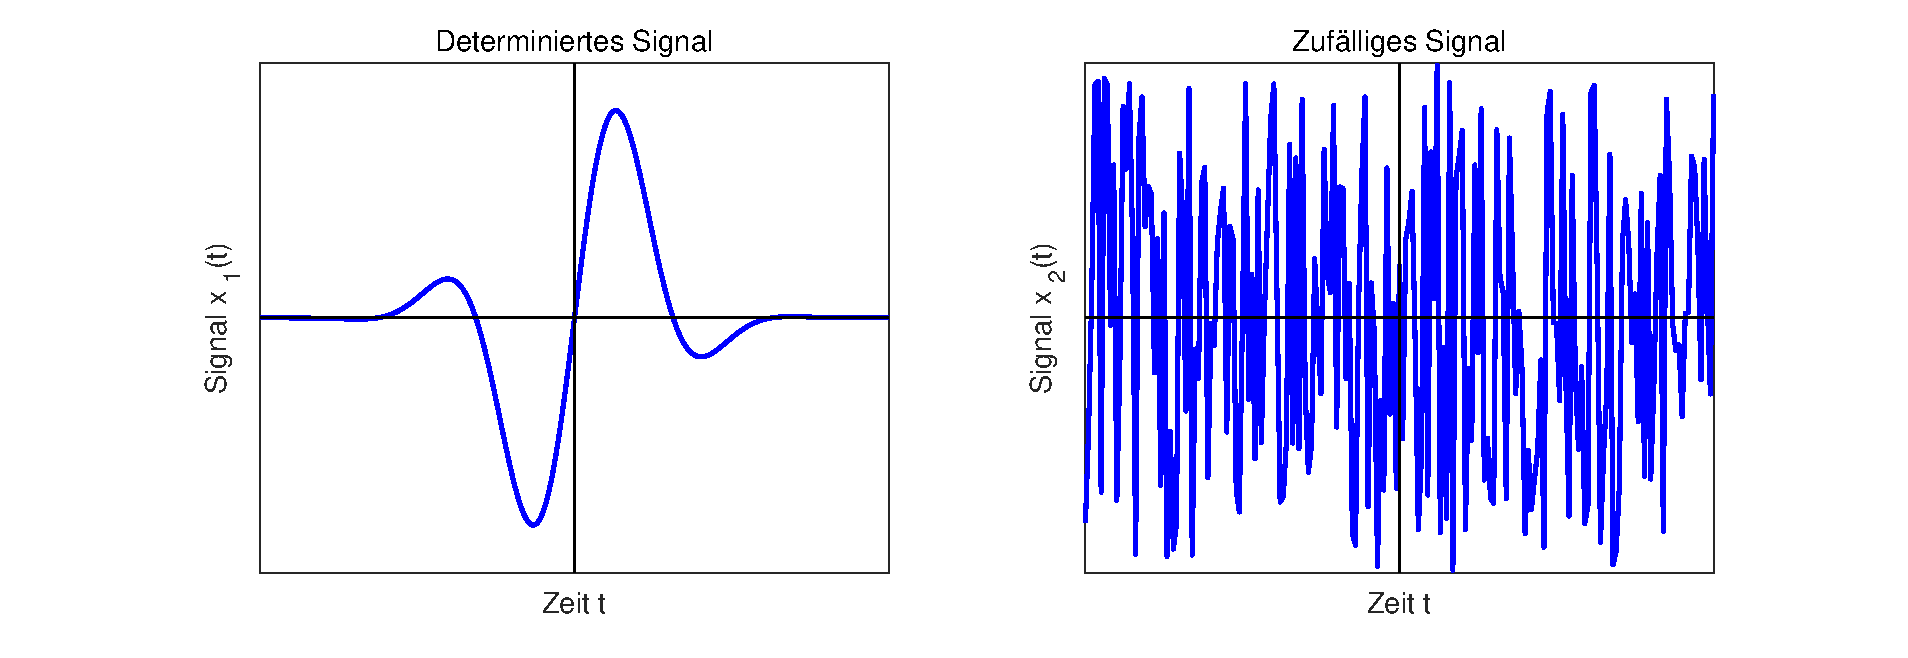
\includegraphics[width=1.0\textwidth]{Kapitel1/Bilder/image2.eps}
  \caption{Beispiele f\"{u}r determinierte und zuf\"{a}llige Signale}
  \label{fig:DeterminierteZuffaeligeSignale}
\end{figure}


\noindent In den Teilen A und B dieser Buchreihe werden determinierte Signale betrachtet. Zuf\"{a}llige Signale werden im Teil C dieser Buchreihe behandelt.


\subsubsection{ Zeitlich begrenzte und kausale Signale}
In der Systemtheorie wird oft mit zeitlich begrenzten Signalen gearbeitet. Ein Grund daf\"{u}r liegt in dem begrenzten Zeitraum, in dem ein System beobachtet werden kann. Ein weiterer Grund ist, dass f\"{u}r die Charakterisierung von Systemen teilweise Testsignale verwendet werden, die Spr\"{u}nge aufweisen. Auch diese Signale sind zumindest einseitig zeitbegrenzt. Bild \ref{fig:BegrenztKausal} zeigt zeitlich begrenzte Signale.


\begin{figure}[H]
  \centerline{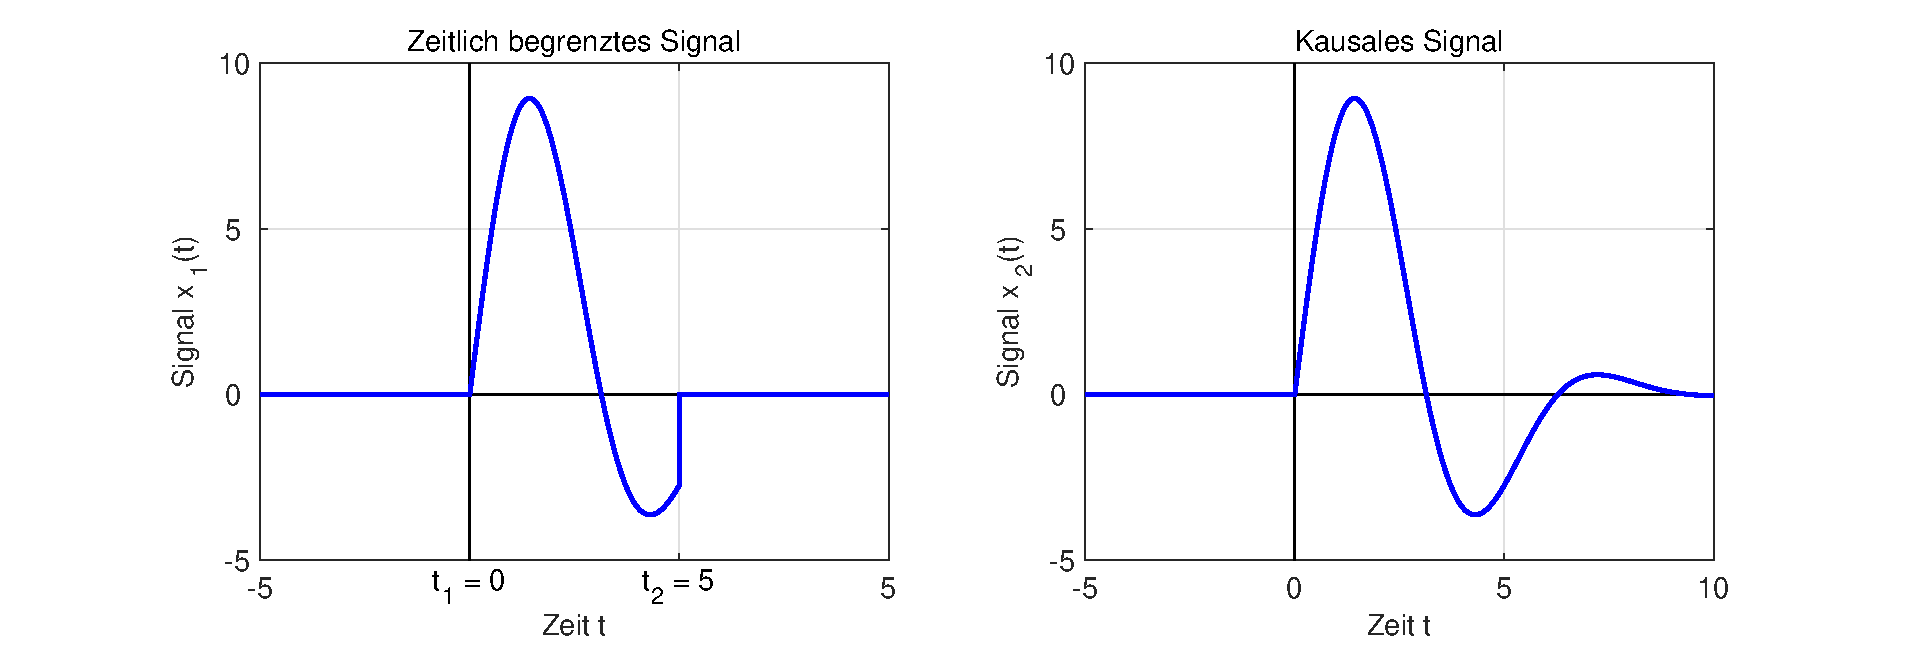
\includegraphics[width=1\textwidth]{Kapitel1/Bilder/image3.eps}}
  \caption{Darstellung eines beidseitig zeitbegrenzten und eines kausalen Signals}
  \label{fig:BegrenztKausal}
\end{figure}


\noindent Signale sind beidseitig zeitbegrenzt Signale, wenn sie nur f\"{u}r einen Zeitraum t${}_{1}$ $\leq$ t $\leq$ t${}_{2}$ von null verschieden sind. Einige Signale sind nur einseitig begrenzt, zum Beispiel ist ein zum Zeitpunkt t = t${}_{1}$ stattfindender Spannungssprung von 0 V auf 1 V nur einseitig zeitbegrenzt. Da diese Signale rechts auf dem Zeitstrahl von null verschieden sind, werden sie als rechtsseitige Signale bezeichnet. 

\noindent Ein kausales Signal ist ein spezielles rechtsseitiges Signal, für das gilt:

\begin{equation}\label{eq:onethree}
x\left(t\right)=0\quad \text{ für } t< 0 
\end{equation}

\noindent Auf die Bedeutung des Begriffes eines kausalen Signals wird bei der Diskussion von kausalen Systemen n\"{a}her eingegangen. 

\subsubsection{ Quadratisch integrierbare Signale}
F\"{u}r die Existenz von uneigentlichen Integralen zum Beispiel bei der Fourier-Transformation sind die Begriffe der Leistungs- und Energiesignale wesentlich. Zur Begriffsdefinition wird von der Vorstellung ausgegangen, dass die an einem Widerstand umgesetzte Leistung p${}_{EL}$(t) proportional zum Quadrat der anliegenden Spannung u(t) ist.


\begin{equation}\label{eq:onefour}
p_{EL} \left(t\right)=\dfrac{u^{2} \left(t\right)}{R} =i^{2} \left(t\right)\cdot R
\end{equation}

\noindent Die in dem Widerstand umgesetzte Energie ergibt sich aus dem Integral der umgesetzten Leistung \"{u}ber der Zeit.

\begin{equation}\label{eq:onefive}
E=\int\limits _{-\infty }^{\infty }p_{EL} \left(t\right) \; dt =\int\limits _{-\infty }^{\infty }\dfrac{u^{2} \left(t\right)}{R} \; dt =\int\limits _{-\infty }^{\infty }i^{2} \left(t\right)\cdot R\;dt 
\end{equation}

\noindent F\"{u}r den Vergleich von Systemen sind vielfach Leistungsverh\"{a}ltnisse von Bedeutung, sodass auf einen konstanten Faktor verzichtet wird. Verallgemeinernd wird die Energie eines Signals definiert als 

\begin{equation}\label{eq:onesix}
E=\int\limits _{-\infty }^{\infty }\left|x\left(t\right)\right|^{2} {\rm \; }dt
\end{equation}

\medskip

{\fontfamily{phv}\selectfont
\noindent\textbf{Energiesignale}} \smallskip

\noindent Energiesignale haben in dem Intervall von - $\infty$ $\mathrm{<}$ t $\mathrm{<}$ $\infty$ eine von Null verschiedene und endliche Gesamtenergie. Die mathematische Bedingung f\"{u}r Energiesignale lautet:

\begin{equation}\label{eq:oneseven}
0<\int\limits _{-\infty }^{\infty }\left|x\left(t\right)\right|^{2} \; dt<\infty
\end{equation}


\noindent Diese Bedingung ist f\"{u}r jedes zeitbegrenzte und amplitudenbegrenzte Signal erf\"{u}llt. Signale, die gleichzeitig zeit- und amplitudenbegrenzt sind, sind damit immer Energiesignale. Die Forderung nach gleichzeitiger Begrenzung von Zeitbereich und Amplitude ist hinreichend, aber nicht unbedingt notwendig.\\

\noindent
\colorbox{lightgray}{%
\arrayrulecolor{white}%
\renewcommand\arraystretch{0.6}%
\begin{tabular}{ wl{16.5cm} }
{\fontfamily{phv}\selectfont
\noindent{Beispiel: Energiesignal}} \smallskip
\end{tabular}%
}\bigskip

\noindent F\"{u}r das Signal x(t) mit  $a >  0$ soll gepr\"{u}ft werden, ob es sich um ein Energiesignal handelt.

\begin{equation}\label{eq:oneeight}
x(t)=e^{\displaystyle -\left|a\cdot t\right|}
\end{equation}

\noindent Das Signal x(t) ist f\"{u}r alle t mit  $-\infty < t < \infty$ definiert und ungleich null. Mit Gleichung \ref{eq:oneeight} errechnet sich die Energie des Signals zu

\begin{equation}\label{eq:onenine}
E=\int\limits _{-\infty }^{\infty }\left|e^{\displaystyle -\left|a\cdot t\right|} \right|^{2} \;  dt=2\cdot \int\limits _{0}^{\infty }e^{\displaystyle -2\cdot a\cdot t}  \;  dt=\left. 2\cdot \dfrac{e^{\displaystyle -2\cdot a\cdot t} }{-2\cdot a} \right|_{0}^{\infty } =2\cdot \dfrac{0-1}{-2\cdot a} =\dfrac{1}{a} 
\end{equation}


\noindent Die Energie des Signals ist endlich, das Signal x(t) ist demnach ein Energiesignal, das zeitlich nicht begrenzt ist. 

\noindent 

\noindent Bei vielen technischen Aufgabenstellungen weisen Signale eine endliche Energie auf, sodass diese Signale in der Systemtheorie von gro{\ss}er Bedeutung sind. Aus mathematischer Sicht handelt es sich bei den Energiesignalen um die Klasse der in dem Intervall von - $\infty$ $\mathrm{<}$ t $\mathrm{<}$ $\infty$ quadratisch integrierbaren Funktionen. \bigskip

{\fontfamily{phv}\selectfont
\noindent\textbf{Leistungssignale}} \smallskip

\noindent Leistungssignale haben im Intervall - $\infty$ $\mathrm{<}$ t $\mathrm{<}$ $\infty$ eine von Null verschiedene und endliche mittlere Leistung. Mathematisch ergibt sich folgende Definition f\"{u}r Leistungssignale:

\begin{equation}\label{eq:oneten}
\lim_{T \to \infty} \dfrac{1}{T}\cdot \int\limits _{-T/2}^{T/2}\left|x(t)\right|^{2} dt <\infty
\end{equation}

\noindent F\"{u}r Signale mit einer begrenzten Amplitude bedeutet das, dass sie nicht zeitbegrenzt sein m\"{u}ssen. Ihre Energie ist zwar unendlich, ihre Energie im Zeitintervall T ist aber begrenzt. 

\clearpage
\noindent
\colorbox{lightgray}{%
\arrayrulecolor{white}%
\renewcommand\arraystretch{0.6}%
\begin{tabular}{ wl{16.5cm} }
{\fontfamily{phv}\selectfont
\noindent{Beispiel: Leistungssignal }}
\end{tabular}%
}\bigskip

\noindent Ein Beispiel f\"{u}r ein Leistungssignal ist das konstante Signal x(t).

\begin{equation}\label{eq:oneeleven}
x\left(t\right)=c
\end{equation}

\noindent Einsetzen der Funktion in die Bedingung f\"{u}r Leistungssignale ergibt

\begin{equation}\label{eq:onetwelve}
\lim_{T \to \infty} \dfrac{1}{T}\cdot \int\limits _{-T/2}^{T/2}\left|x(t)\right|^{2} dt 
=\lim_{T \to \infty} \dfrac{1}{T}\cdot \int\limits _{-T/2}^{T/2}\left|c\right|^{2} dt 
=\lim_{T \to \infty} \dfrac{1}{T}\cdot T\cdot \left|c\right|^{2} =\left|c\right|^{2} <\infty
\end{equation}


\noindent Der Wert des Integrals ist endlich, sodass das Signal x(t) ein Leistungssignal ist. Die Energie des Signals ist unendlich, sodass das konstante Signal kein Energiesignal ist.

\begin{equation}\label{eq:onethirteen}
E=\int\limits _{-\infty }^{\infty }c^{2} \;  dt=c^{2} \cdot \int\limits _{-\infty }^{\infty }1 \;  dt=\infty
\end{equation}

\noindent Ein Vergleich der Definitionen von Leistungs- und Energiesignalen zeigt, dass ein Energiesignal stets ein Leistungssignal ist. Ist die Energie eines Signals endlich, gilt die Beziehung

\begin{equation}\label{eq:onefourteen}
\int\limits _{-\infty }^{\infty }\left|x\left(t\right)\right|^{2} \; dt=\lim_{T \to \infty}  \, \, \int\limits _{-T/2}^{T/2}\left|x\left(t\right)\right|^{2} \; dt<\infty
\end{equation}


\noindent Daraus folgt f\"{u}r die Leistung des Signals

\begin{equation}\label{eq:onefifteen}
\lim_{T \to \infty}  \, \, \dfrac{1}{T} \cdot \int\limits _{-T/2}^{T/2}\left|x(t)\right|^{2} \; dt=0
\end{equation}


\noindent Signale, die weder Energie- noch Leistungssignale sind, spielen in der Systemtheorie nur in Sonderf\"{a}llen eine Rolle, da die Systemtheorie technische Vorg\"{a}nge beschreibt, die grunds\"{a}tzlich mit einer endlichen Leistung verbunden sind.


\subsubsection{ Symmetrieeigenschaften zeitkontinuierlicher Signale}

\noindent Die Interpretation von Signalen vereinfacht sich, wenn ihre Symmetrieeigenschaften bekannt sind. Gerade und ungerade Signale weisen eine derartige Symmetrie auf. Gerade Signale sind f\"{u}r alle t symmetrisch zur Achse t = 0, also zur Ordinatenachse. F\"{u}r ein gerades Signal gilt deshalb die Bedingung: 

\begin{equation}\label{eq:onesixteen}
x(t)=x(-t)
\end{equation}


\noindent Ein kosinusf\"{o}rmiges Signal ist Beispiel f\"{u}r ein gerades Signal, denn es gilt:

\begin{equation}\label{eq:oneseventeen}
x_{1} \left(t\right)=\cos \left(\omega \cdot t\right)=\cos \left(-\omega \cdot t\right)=x_{1} \left(-t\right)
\end{equation}

\noindent Ungerade Signale sind f\"{u}r alle t punktsymmetrisch zu dem Koordinatenursprung. Diese Bedingung kann mathematisch ausgedr\"{u}ckt werden als

\begin{equation}\label{eq:oneeighteen}
x\left(t\right)=-x\left(-t\right)
\end{equation}

\noindent Ein sinusf\"{o}rmiges Signal ist ein Beispiel f\"{u}r ein ungerades Signal, denn es gilt:

\begin{equation}\label{eq:onenineteen}
x_{2} \left(t\right)=\sin \left(\omega \cdot t\right)=-\sin \left(-\omega \cdot t\right)=-x_{2} \left(-t\right)
\end{equation}


\noindent Bild \ref{fig:SymmetrieSinusKosinus} zeigt Kosinus- und Sinusfunktionen als Beispiele f\"{u}r gerade und ungerade Signale. Die Bedingung f\"{u}r gerade und ungerade Signale ist rot gestrichelt eingezeichnet.
\clearpage

\begin{figure}[H]
  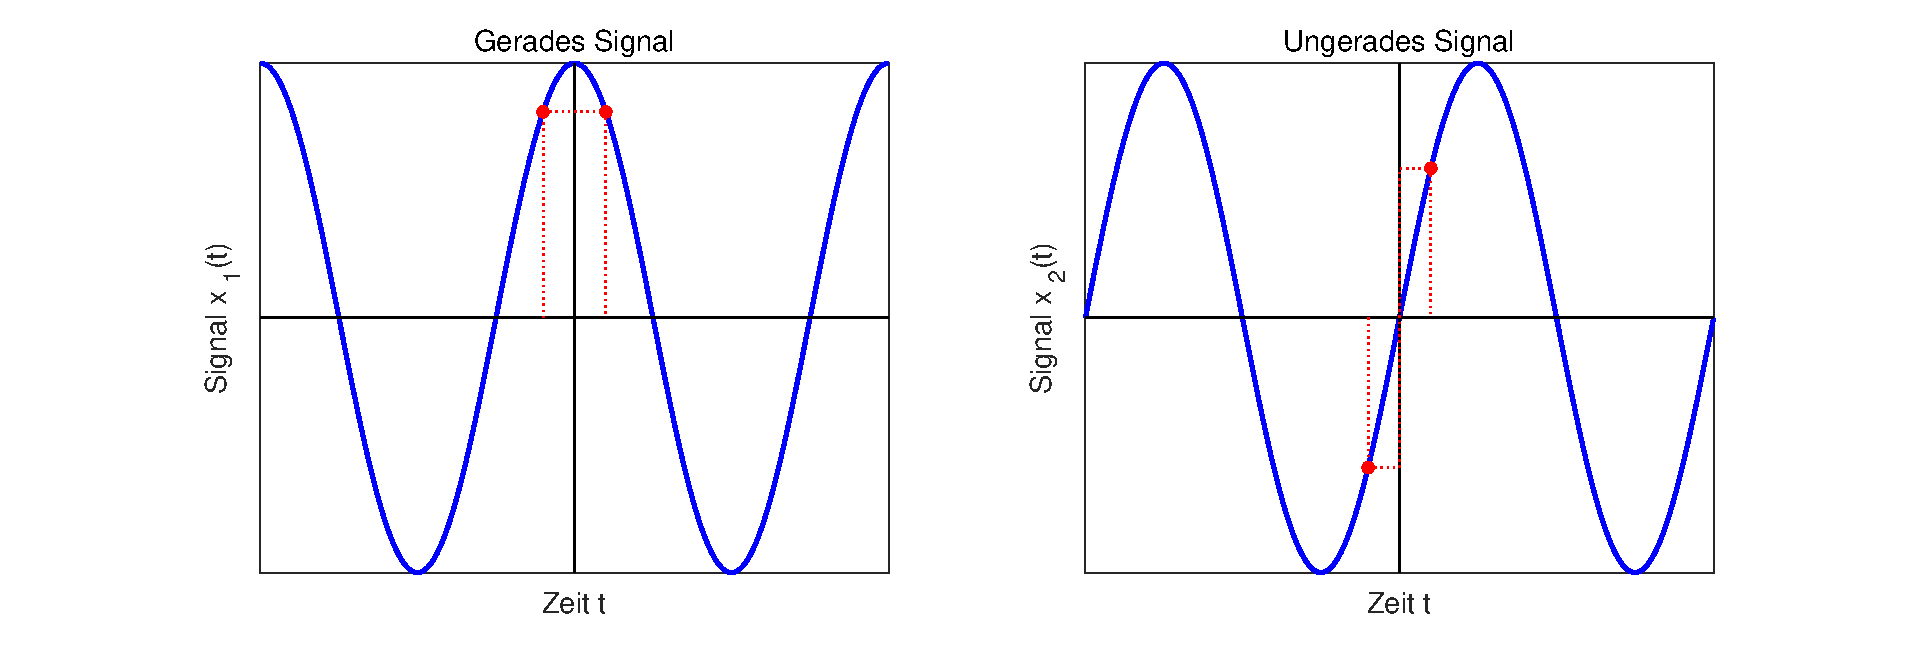
\includegraphics[width=1\textwidth]{Kapitel1/Bilder/image4}
  \caption{Kosinus- und Sinusfunktionen als Beispiele f\"{u}r gerade und ungerade Signale}
  \label{fig:SymmetrieSinusKosinus}
\end{figure}

\noindent Es existieren Signale, die weder gerade, noch ungerade sind, sie weisen keine Symmetrie auf. Jedes beliebige Signal l\"{a}sst sich aber in einen geraden Signalanteil x${}_{G}$(t) und einen ungeraden Signalanteil x${}_{U}$(t) aufspalten. 

\begin{equation}\label{eq:onetwenty}
x\left(t\right)=x_{G} \left(t\right)+x_{U} \left(t\right)
\end{equation}


\noindent wobei sich die beiden Anteile ergeben aus

\begin{equation}\label{eq:onetwentyone}
x_{G} \left(t\right)=\dfrac{1}{2} \cdot \left(x\left(t\right)+x\left(-t\right)\right)
\end{equation}


\noindent und 

\begin{equation}\label{eq:onetwentytwo}
x_{U} \left(t\right)=\dfrac{1}{2} \cdot \left(x\left(t\right)-x\left(-t\right)\right)
\end{equation}


\noindent Bild \ref{fig:GeradeUngerade} verdeutlicht die Zerlegung eines Signals in einen geraden und einen ungeraden Anteil an einem Beispiel.

\begin{figure}[H]
  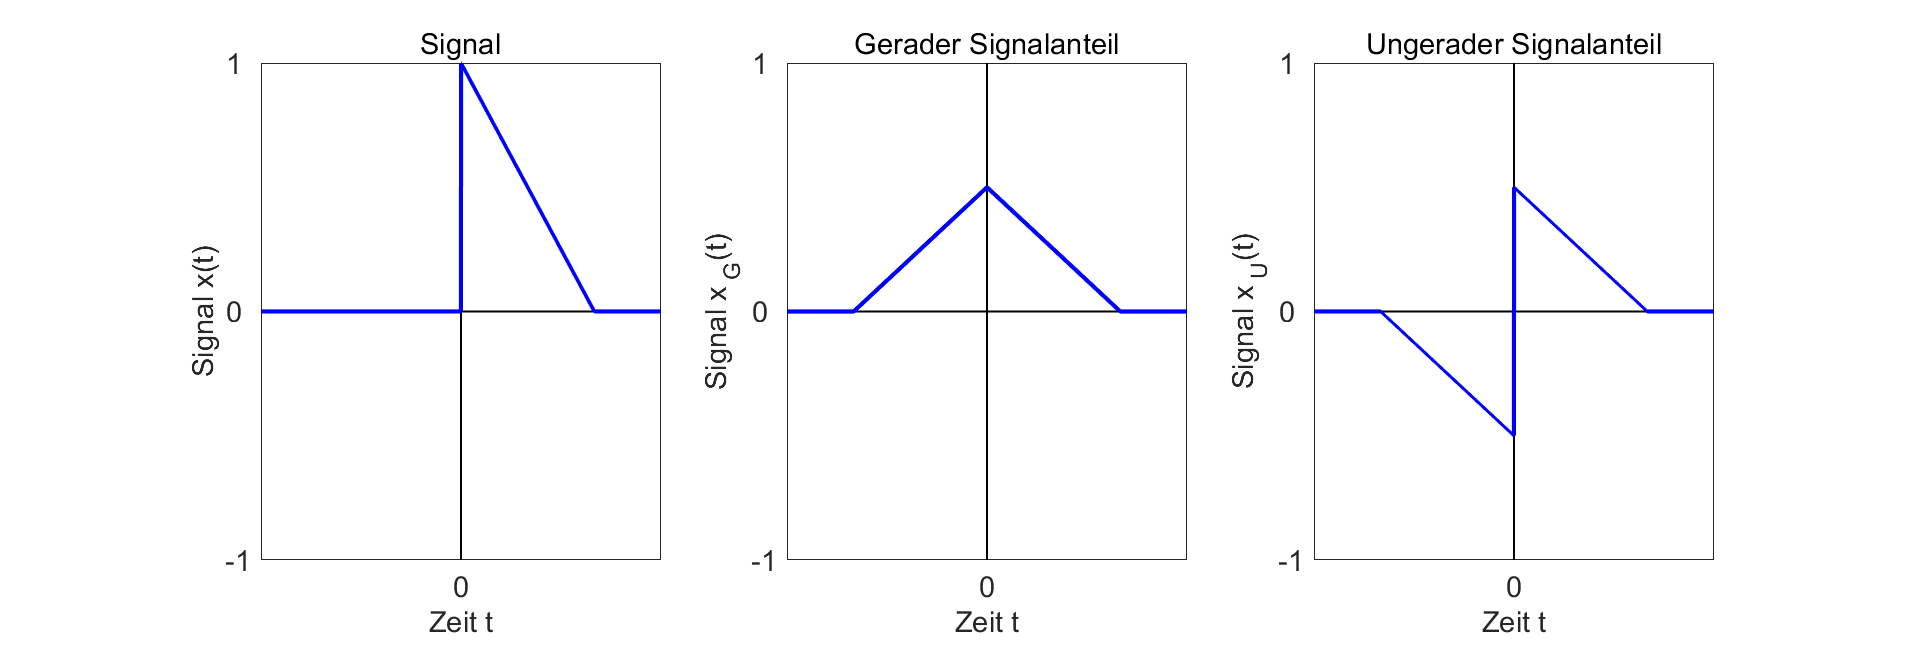
\includegraphics[width=1.0\textwidth]{Kapitel1/Bilder/image5}
  \caption{Zerlegung eines Signals in geraden und ungeraden Anteil}
  \label{fig:GeradeUngerade}
\end{figure}

\noindent Neben der Symmetrie reeller Signale wird zum Beispiel bei der Fourier-Transformation ein konjugiert symmetrisches Signal x*(t) verwendet. Ein Signal ist konjugiert symmetrisch, wenn die Beziehung 

\begin{equation}\label{eq:onetwentythree}
x(t)=x^{*} (-t)
\end{equation}

\noindent gilt.

\clearpage

\subsubsection{ Zusammenfassung Signaleigenschaften}

\noindent Zur besseren Übersicht sind in die Signaleigenschaften für zeit- und wertkontinuierliche Signale dargestellt. 


\begin{table}[H]
\setlength{\arrayrulewidth}{.1em}
\caption{Tabellarische Übersicht über Signaleigenschaften für zeit- und wertkontinuierliche Signale}

\setlength{\fboxsep}{0pt}%
\colorbox{lightgray}{%
\arrayrulecolor{white}%
\begin{tabular}{| l | l |}
\hline
\parbox[c][0.3in][c]{3in}{\smallskip\centering\textbf{\fontfamily{phv}\selectfont{Signaleigenschaft}}} & \parbox[c][0.3in][c]{3in}{\smallskip\centering\textbf{\fontfamily{phv}\selectfont{Mathematische Beschreibung}}}\\ \hline
\parbox[c][1in][c]{3in}{\smallskip\centering{\fontfamily{phv}\selectfont{Explizit definiertes Signal}}} & \parbox[c][1in][c]{3in}{\centering{\fontfamily{phv}\selectfont{Funktionswert kann direkt abgelesen werden,\\zum Beispiel\\[3pt]
$x(t)=10\cdot e^{\displaystyle -a\cdot t^{2}}\cdot\sin (b\cdot t)$}}}\\ \hline

\parbox[c][1in][c]{3in}{\centering{\fontfamily{phv}\selectfont{Implizit definiertes Signal}}} & \parbox[c][1in][c]{3in}{\centering{\fontfamily{phv}\selectfont{Funktionswert muss unter Ber\"{u}cksichtigung von Anfangsbedingungen berechnet werden, zum Beispiel\newline 
$\dfrac{dx}{dt} \; +3\cdot \dfrac{d^{2} x(t)}{dt^{2}} =5\cdot x(t)+\sin (\omega \cdot t)$}}}\\ \hline

\parbox[c][0.64in][c]{3in}{\centering{\fontfamily{phv}\selectfont{Begrenztes Signal}}} & \parbox[c][0.64in][c]{3in}{\centering{\fontfamily{phv}\selectfont{$x(t)=0$ \quad für $t<t_{1} $  und/oder  $ t>t_{2} $}}}\\ \hline

\parbox[c][0.64in][c]{3in}{\centering{\fontfamily{phv}\selectfont{Kausales Signal}}} & \parbox[c][0.64in][c]{3in}{\centering{\fontfamily{phv}\selectfont{$x(t)=0 $ für $t<0$}}}\\ \hline

\parbox[c][0.64in][c]{3in}{\centering{\fontfamily{phv}\selectfont{Energiesignal}}} & \parbox[c][0.64in][c]{3in}{\centering{\fontfamily{phv}\selectfont{$0<\int\limits _{-\infty }^{\infty }\left|x(t)\right|^{2} \; dt<\infty  $}}}\\ \hline

\parbox[c][0.64in][c]{3in}{\centering{\fontfamily{phv}\selectfont{Leistungssignal}}} & \parbox[c][0.64in][c]{3in}{\centering{\fontfamily{phv}\selectfont{$\lim\limits_{T\to \infty} \; \dfrac{1}{T} \cdot \int\limits _{-T/2}^{T/2}\left|x(t)\right|^{2} dt<\infty  $}}}\\ \hline

\parbox[c][0.64in][c]{3in}{\centering{\fontfamily{phv}\selectfont{Gerades Signal}}} & \parbox[c][0.64in][c]{3in}{\centering{\fontfamily{phv}\selectfont{$x(t)=x(-t)$}}}\\ \hline

\parbox[c][0.64in][c]{3in}{\centering{\fontfamily{phv}\selectfont{Ungerades Signal}}} & \parbox[c][0.64in][c]{3in}{\centering{\fontfamily{phv}\selectfont{$x(t)=-x(-t)$}}}\\ 
\hline

\parbox[c][0.64in][c]{3in}{\centering{\fontfamily{phv}\selectfont{Gerader Signalanteil}}} & \parbox[c][0.64in][c]{3in}{\centering{\fontfamily{phv}\selectfont{$x_{G} (t)=\dfrac{1}{2} \cdot (x(t)+x(-t))$}}}\\ 
\hline

\parbox[c][0.64in][c]{3in}{\centering{\fontfamily{phv}\selectfont{Ungerader Signalanteil}}} & \parbox[c][0.64in][c]{3in}{\centering{\fontfamily{phv}\selectfont{$x_{U} (t)=\dfrac{1}{2} \cdot \left(x(t)-x(-t)\right)$}}}\\ 
\hline

\parbox[c][0.64in][c]{3in}{\centering{\fontfamily{phv}\selectfont{Konjugiert symmetrisches Signal}}} & \parbox[c][0.64in][c]{3in}{\centering{\fontfamily{phv}\selectfont{$x(t)=x^{*} (-t)$}}}\\ 
\hline
\end{tabular}%
}
\label{tab:oneone}
\end{table}

\clearpage


\subsection{ Rechnen mit Sprung- und Impulsfunktion}


\subsubsection{ Allgemein}

\noindent Die Beschreibung und Interpretation von Systemen kann unter anderem \"{u}ber die Systemreaktion auf standardisierte Eingangssignale erfolgen. Deshalb werden in diesem Abschnitt Sprung- und Impulsfunktionen vorgestellt, weitere Funktionen daraus abgeleitet und das Rechnen mit Impulsfunktionen vertieft.


\subsubsection{ Sprungfunktion}

\noindent Die Sprungfunkton $\sigma$(t) ist als Grenzwert einer Funktion $\sigma$(t) definiert, die ihren Funktionswert in einem Zeitraum der Länge $\varepsilon$ von 0 auf 1 wechselt. Die Funktion $\sigma$(t) wird im Folgenden als verallgemeinerte Sprungfunktion $\sigma$(t) bezeichnet. Sie ist abschnittsweise definiert als 

\begin{equation}\label{eq:onetwentyfour}
\sigma _{\varepsilon} (t)=\left\{\begin{array}{ll}
{0 \qquad \quad \text{ für } t<-\varepsilon /2} \\
{\dfrac{1}{\varepsilon } \cdot  t +\dfrac{1}{2} \;\, \text{ für} -\varepsilon /2<t<\varepsilon /2} \\
{1 \qquad \quad \text{ für } \varepsilon /2 \le t} \end{array}\right.
\end{equation}


\noindent Ihr Funktionsverlauf ist Bild \ref{fig:NaeherungSprungfunktion} dargestellt.

\begin{figure}[H]
  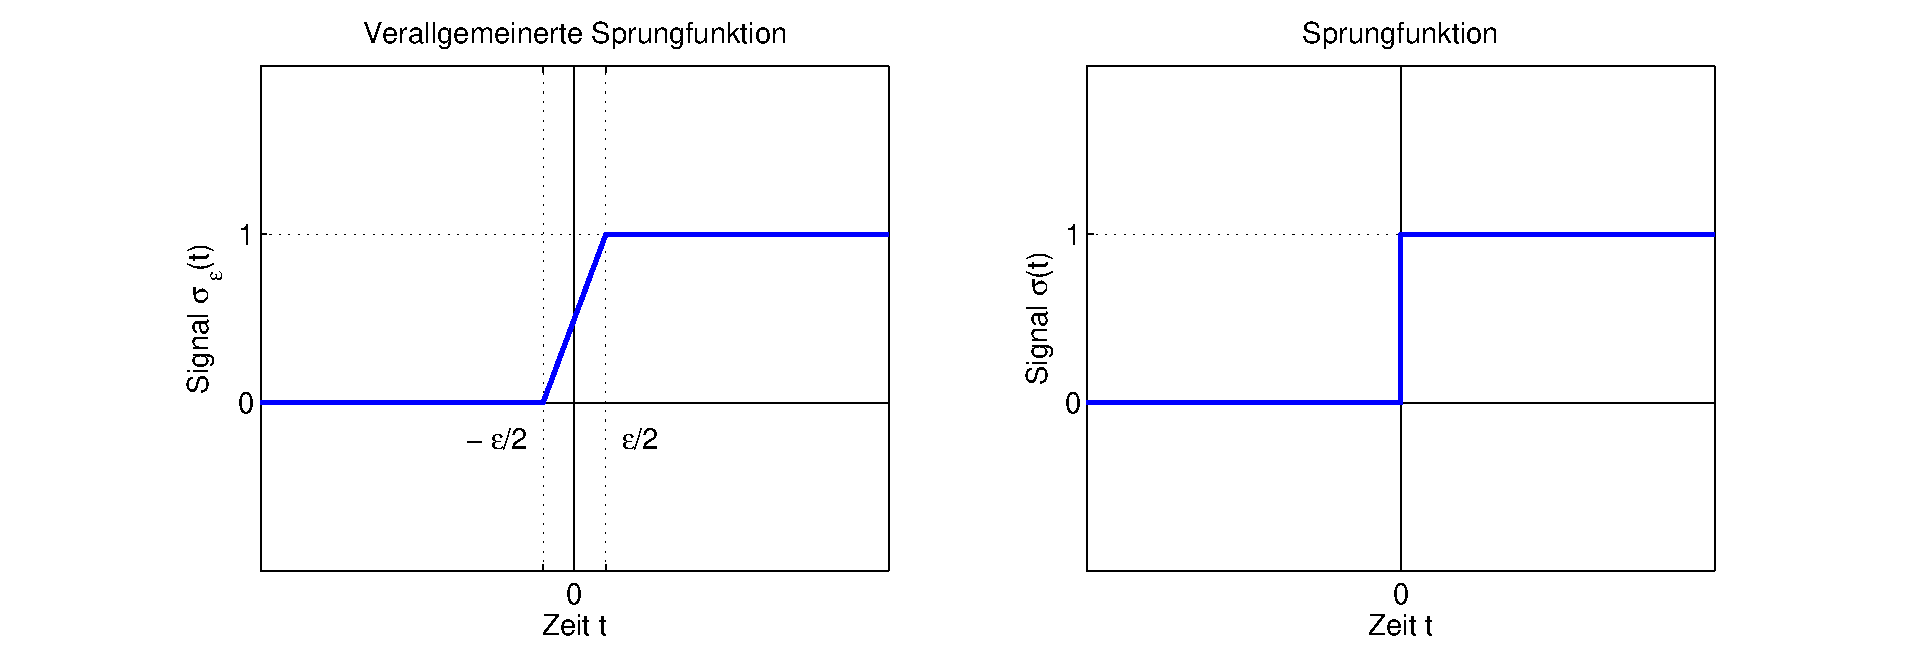
\includegraphics[width=1.0\textwidth]{Kapitel1/Bilder/image6.eps}
  \caption{Verallgemeinerte Sprungfunktion $\sigma$(t)}
  \label{fig:NaeherungSprungfunktion}
\end{figure}


\noindent Mit kleiner werdender Breite $\varepsilon$ wird der \"{U}bergang immer steiler. \"{U}ber eine Grenzwertbetrachtung $\epsilon$ $\rightarrow$ 0 geht die Funktion $\sigma$(t) in die Sprungfunktion $\sigma$(t) \"{u}ber, die an der Stelle t = 0 von 0 auf 1 springt. Die Sprungfunktion $\sigma$(t) ist abschnittsweise definiert als

\begin{equation}\label{eq:onetwentyfive}
x\left(t\right)=\sigma \left(t\right)=\left\{\begin{array}{l} 
{0\qquad \text{für } t<0} \\ 
{1\qquad \text{für } t \ge 0} 
\end{array}\right.\\
\end{equation}


\noindent F\"{u}r den Zeitpunkt t = 0 existieren in der Literatur unterschiedliche Definitionen. Im Hinblick auf diskrete Signale wird hier f\"{u}r den Zeitpunkt t = 0 der Funktionswert $\sigma$(t = 0) = 1 gew\"{a}hlt. 

\noindent Bei der Diskussion der Sprungstelle wird oftmals von rechtsseitigem und linksseitigem Grenzwert gesprochen. Der linksseitige Grenzwert wird als $\sigma$(0${}_{-}$) bezeichnet. Er hat den Wert der Funktion kurz vor dem Sprung $\sigma$(0${}_{-}$) = 0. Der rechtsseitige Grenzwert wird als $\sigma$(0${}_{+}$) bezeichnet. Er hat den Wert der Funktion kurz nach dem Sprung $\sigma$(0${}_{+}$) = 1. 

\noindent Die Sprungfunktion wird auch als Heaviside-Funktion bezeichnet. Sie wird zum Beispiel daf\"{u}r verwendet, Einschaltvorg\"{a}nge zu beschreiben. Die Sprungfunktion ist zeitlich nicht begrenzt, und sie ist kein Energiesignal. Wegen ihrer konstanten Amplitude ist die Bedingung f\"{u}r ein Leistungssignal erf\"{u}llt. Da die Sprungfunktion f\"{u}r t $\mathrm{<}$ 0 null ist, ist sie eine kausale Funktion.


\subsubsection{ Rechteckfunktion}

\noindent Die Rechteckfunktion ist abschnittsweise definiert als 

\begin{equation}\label{eq:onetwentysix}
x\left(t\right)=\left\{\begin{array}{l} 
{0\qquad \text{für }t<-T} \\ 
{1\qquad \text{für }-T{\le t<T}} \\ 
{0\qquad \text{für }T \le t} 
\end{array}\right.
\end{equation}


\noindent Die Rechteckfunktion ist eine Funktion mit endlicher Amplitude und endlicher Dauer. Die Bedingung f\"{u}r ein Energiesignal ist deshalb erf\"{u}llt. Die Funktion repr\"{a}sentiert damit ein Energie- und Leistungssignal. Sie ist nach Gleichung \ref{eq:onetwentysix} aber keine kausale Funktion, da sie f\"{u}r t $\mathrm{<}$ 0 nicht null ist. Durch eine Verschiebung um den Zeitraum T nach rechts kann die Rechteckfunktion in eine kausale Funktion \"{u}berf\"{u}hrt werden. Beide Funktionen sind in Bild \ref{fig:Rechteck} dargestellt.

\begin{figure}[ht]
  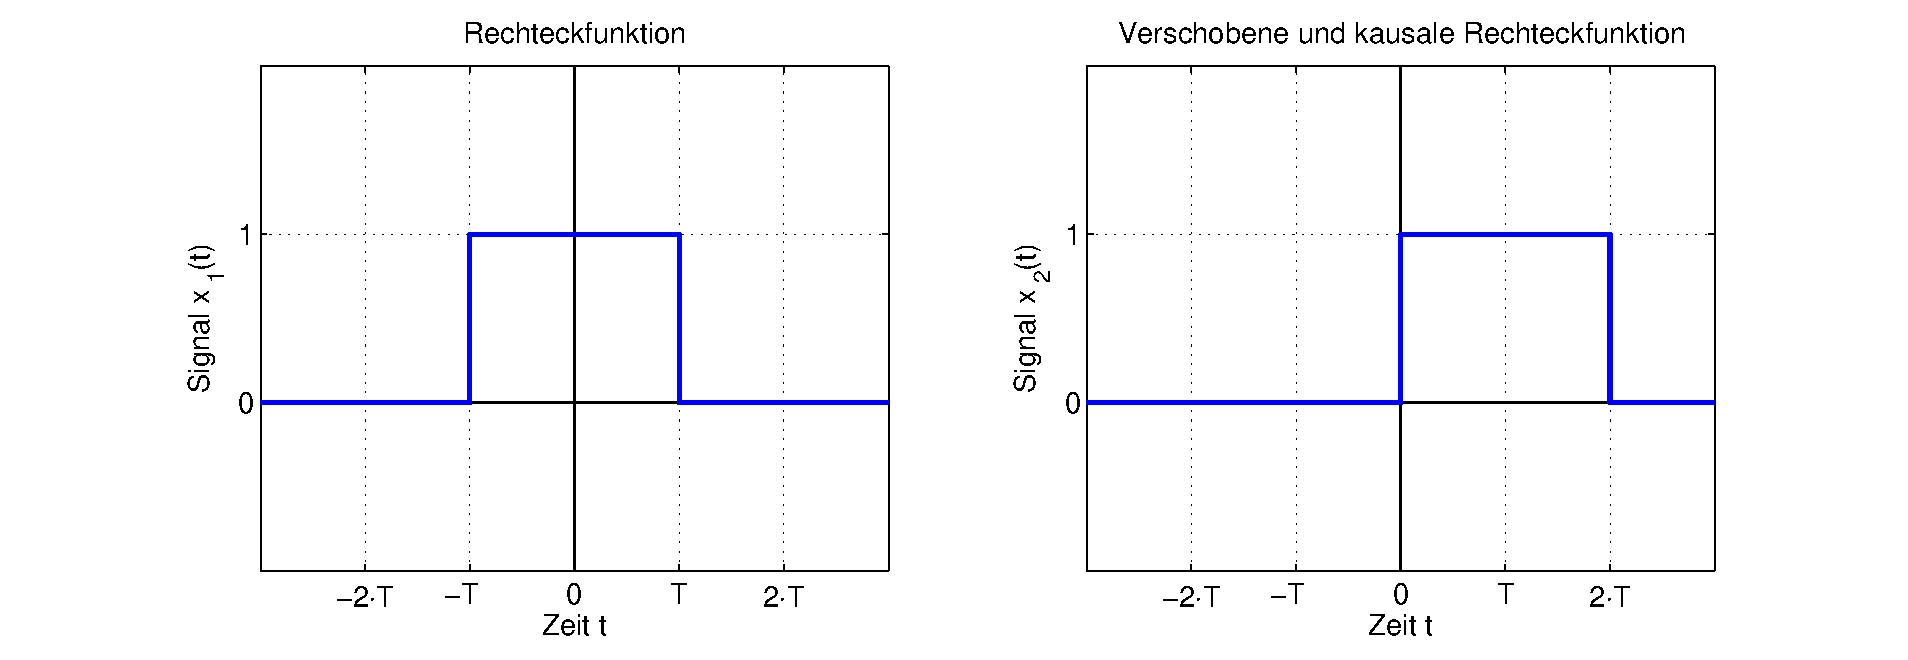
\includegraphics[width=1.0\textwidth]{Kapitel1/Bilder/image7}
  \caption{Rechteckfunktion und verschobene Rechteckfunktion}
  \label{fig:Rechteck}
\end{figure}


\noindent Die Rechteckfunktion kann neben der abschnittsweisen Definition auch als Summe zweier Sprungfunktionen dargestellt werden, die um - T beziehungsweise + T verschoben sind.

\begin{equation}\label{eq:onetwentyseven}
x_{1} \left(t\right)=\sigma \left(t+T\right)-\sigma \left(t-T\right)
\end{equation}


\noindent Entsprechend gilt f\"{u}r die kausale Rechteckfunktion

\begin{equation}\label{eq:onetwentyeight}
x_{2} \left(t\right)=\sigma \left(t\right)-\sigma \left(t-2\cdot T\right)
\end{equation}


\subsubsection{ Signum-Funktion }

\noindent Die Signum-Funktion sgn(t) ist abschnittsweise definiert als


\begin{equation}\label{eq:onetwentynine}
x(t)=sgn(t)=\left\{\begin{array}{l} {-{\rm 1\; }\quad \text{für } t<0} \\ 
{+1{\rm \; }\quad \text{für } 0 \le {\rm t\; }} \end{array}\right.
\end{equation}

\noindent Auch die Signum-Funktion kann mithilfe der Sprungfunktion dargestellt werden.

\begin{equation}\label{eq:onethirty}
x(t)=sgn(t)=2\cdot \sigma (t)-1
\end{equation}


\noindent Bild \ref{fig:Signum} stellt die Signum-Funktion grafisch dar. Sie ist unendlich lange ungleich null und ist kein Energiesignal. Wegen ihrer konstanten Amplitude ist die Bedingung f\"{u}r ein Leistungssignal erf\"{u}llt. Die Signum-Funktion ist nicht kausal und kann durch eine zeitliche Verschiebung auch nicht in ein kausales Signal \"{u}berf\"{u}hrt werden.


\begin{figure}[ht]
  \centerline{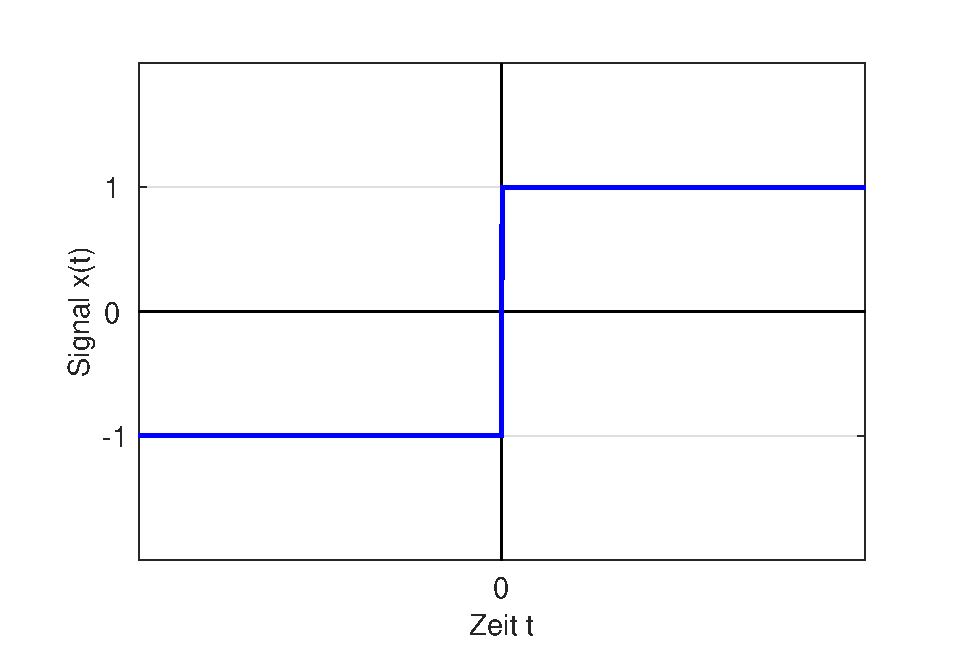
\includegraphics[width=0.5\textwidth]{Kapitel1/Bilder/image8.eps}}
  \caption{Signum-Funktion sgn(t)}
  \label{fig:Signum}
\end{figure}

\subsubsection{Rampenfunktion}

\noindent Ideale Sprung-, Rechteck- und Signum-Funktionen werden als Testsignale verwendet. Praktisch lassen sie sich wegen der unendlich gro{\ss}en Signal\"{a}nderung an den Unstetigkeitsstellen allerdings nur n\"{a}herungsweise realisieren. Au{\ss}erdem k\"{o}nnen Systeme, die mit einem sprungf\"{o}rmigen Signal angeregt werden, zerst\"{o}rt werden. Zum Beispiel werden die Schaufeln eines Turbinenrades, das sprungf\"{o}rmig mit einem gro{\ss}en Volumenstrom beaufschlagt wird, brechen. Die Rampenfunktion bietet einen stetigen \"{U}bergang der Funktionswerte f\"{u}r den Zeitraum t $\mathrm{<}$ 0 und den Zeitraum t $\mathrm{\ge}$ 0. Die Rampenfunktion ist definiert als

\begin{equation}\label{eq:onethirtyone}
x(t)=\left\{\begin{array}{ll} 
{0 \quad \text{ für }t<0} \\ 
{t \quad \text{ für }t \ge 0} 
\end{array}\right.
\end{equation}


\noindent Bild \ref{fig:Rampenfunktion} stellt die Rampenfunktion grafisch dar.

\begin{figure}[ht]
  \centerline{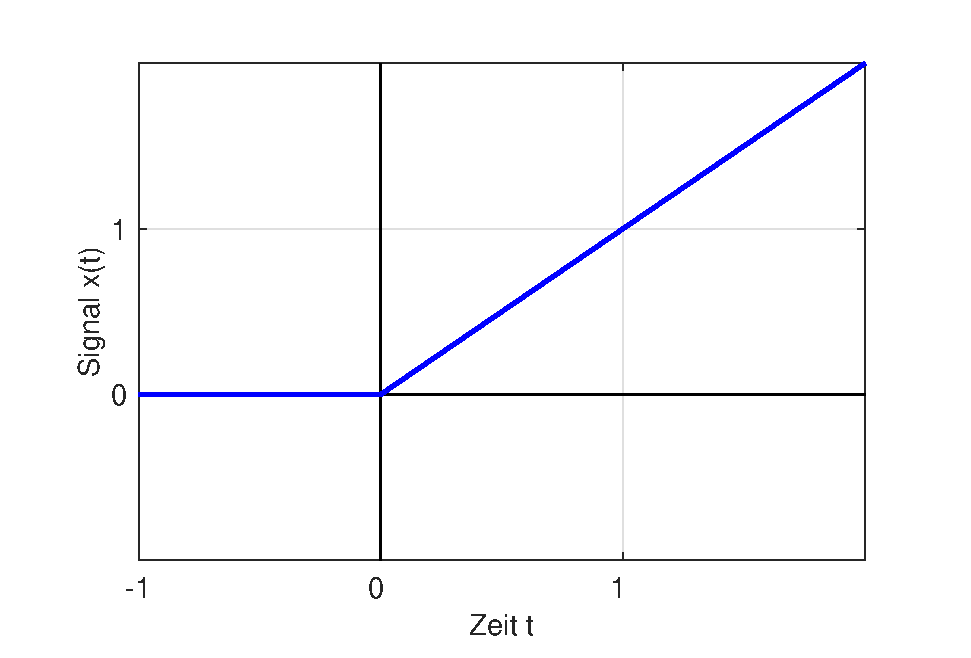
\includegraphics[width=0.5\textwidth]{Kapitel1/Bilder/image9}}
  \caption{Rampenfunktion}
  \label{fig:Rampenfunktion}
\end{figure}


\noindent Die Rampenfunktion kann sowohl als Integral der Sprungfunktion 

\begin{equation}\label{eq:onethirtytwo}
x\left(t\right)=\int\limits _{-\infty }^{t}\sigma \left(\tau \right) \;d\tau = \left\{\begin{array}{l} {0\qquad \text{für } t < 0} \\ 
{t\qquad \text{für } 0\le t} 
\end{array}\right.
\end{equation}


\noindent als auch als Produkt von Sprungfunktion und Zeit t dargestellt werden.

\begin{equation}\label{eq:onethirtythree}
x\left(t\right)=t\cdot \sigma \left(t\right)
\end{equation}


\noindent Die Rampenfunktion hat weder eine begrenzte Amplitude, noch eine begrenzte Zeitdauer, sie ist weder Energie- noch Leistungssignal. Eine ideale Rampenfunktion kann in realen Systemen deshalb nur f\"{u}r einen begrenzten Zeitraum realisiert werden. Da die Rampenfunktion f\"{u}r t $\mathrm{<}$ 0 null ist, beschreibt sie ein kausales Signal.


\subsubsection{ Dreieckfunktion}

\noindent Die Dreieckfunktion ist in Bild 1.10 dargestellt und definiert als

\begin{equation}\label{eq:onethirtyfour}
x\left(t\right)=\left\{\begin{array}{l} 
{0 \qquad \qquad \text{für } t<-T} \\ 
{1+t/T  \quad \,\: \text{ für } -T\le t<0} \\ 
{1-t/T  \quad \,\: \text{ für }  0\le t<T} \\ 
{0 \qquad \qquad \text{für } T\le t} 
\end{array}\right.
\end{equation}


\noindent Bild \ref{fig:DreieckFunktion} stellt eine Dreieckfunktion und eine verschobene Dreieckfunktion grafisch dar.

\begin{figure}[ht]
  \centerline{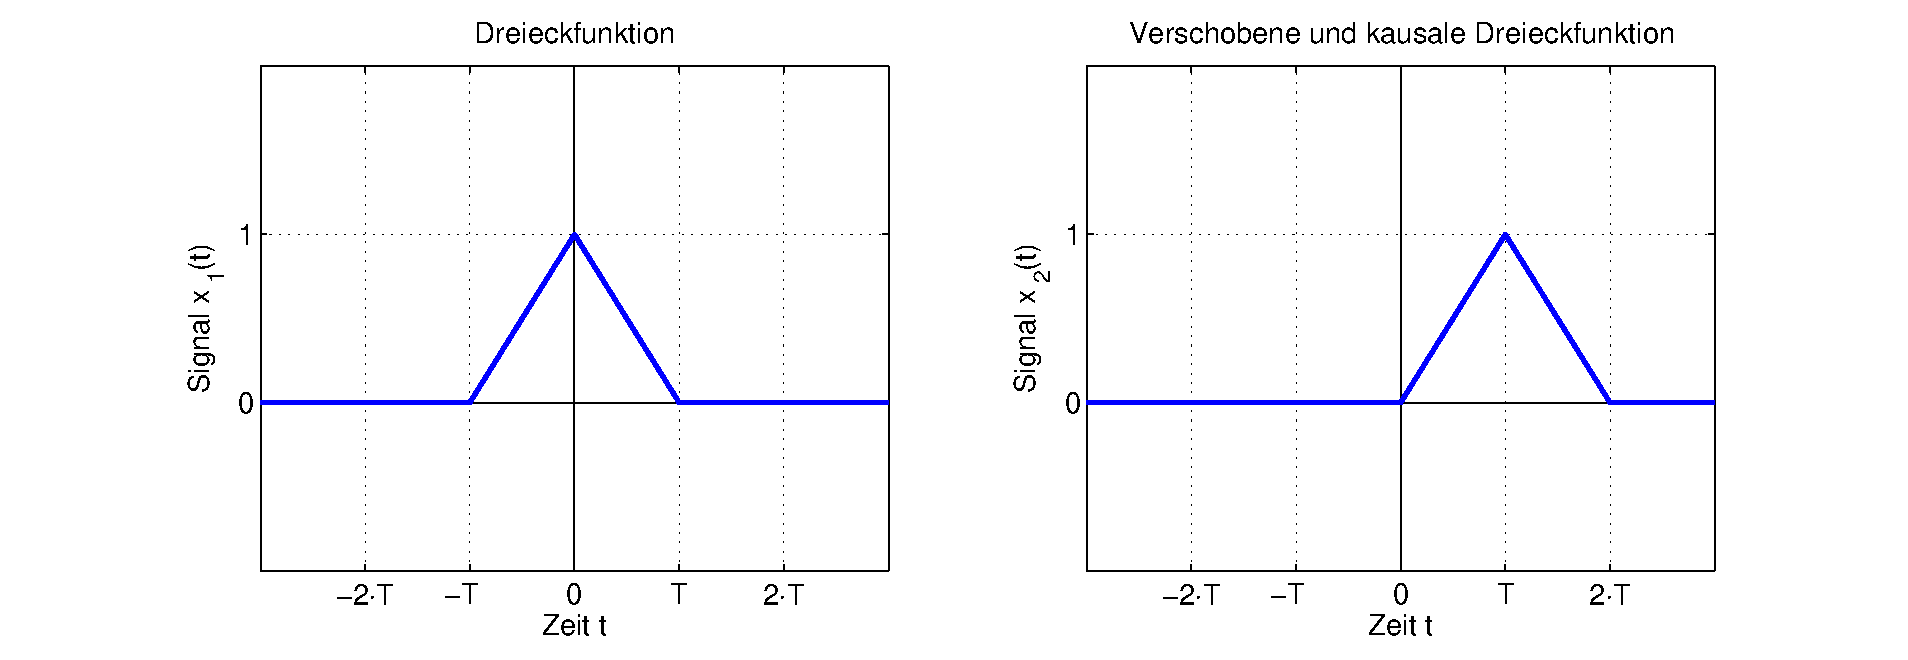
\includegraphics[width=0.9\textwidth]{Kapitel1/Bilder/image10.eps}}
  \caption{Dreieckfunktion und verschobene Dreieckfunktion}
  \label{fig:DreieckFunktion}
\end{figure}

\noindent Die Dreieckfunktion ist eine Funktion mit endlicher Amplitude und endlicher Dauer. Die Bedingung f\"{u}r ein Energiesignal ist erf\"{u}llt. Die Dreieckfunktion ist damit ein Energie- und Leistungssignal. Wie die Rechteckfunktion beginnt die Dreieckfunktion bereits f\"{u}r t = - T. Sie ist deshalb nicht kausal, kann aber durch Verschiebung um den Zeitraum T nach rechts in ein kausales Signal \"{u}berf\"{u}hrt werden.

\noindent Die Dreieckfunktion kann auf unterschiedliche Art aus den bereits dargestellten Funktionen gewonnen werden, zum Beispiel durch \"{U}berlagerung von drei Rampenfunktionen. 

\clearpage

\subsubsection{ Impulsfunktion}

\noindent Von gro{\ss}er Bedeutung f\"{u}r die theoretische Charakterisierung von Systemen ist die Impulsfunktion $\delta$(t). Die Impulsfunktion ist als Grenzwert einer Rechteckfunktion $\delta$(t) definiert, die eine Breite $\epsilon$ und der H\"{o}he 1/$\epsilon$ aufweist. Bild \ref{fig:NaehrungImpulsfunktion} zeigt den Rechteckimpuls.


\begin{equation}\label{eq:onethirtyfive}
\delta _{\varepsilon }(t)=\dfrac{1}{\varepsilon } \cdot \left(\sigma \left(t+\dfrac{\varepsilon }{2} \right)-\sigma \left(t-\dfrac{\varepsilon }{2} \right)\right)
\end{equation}

\begin{figure}[ht]
  \centerline{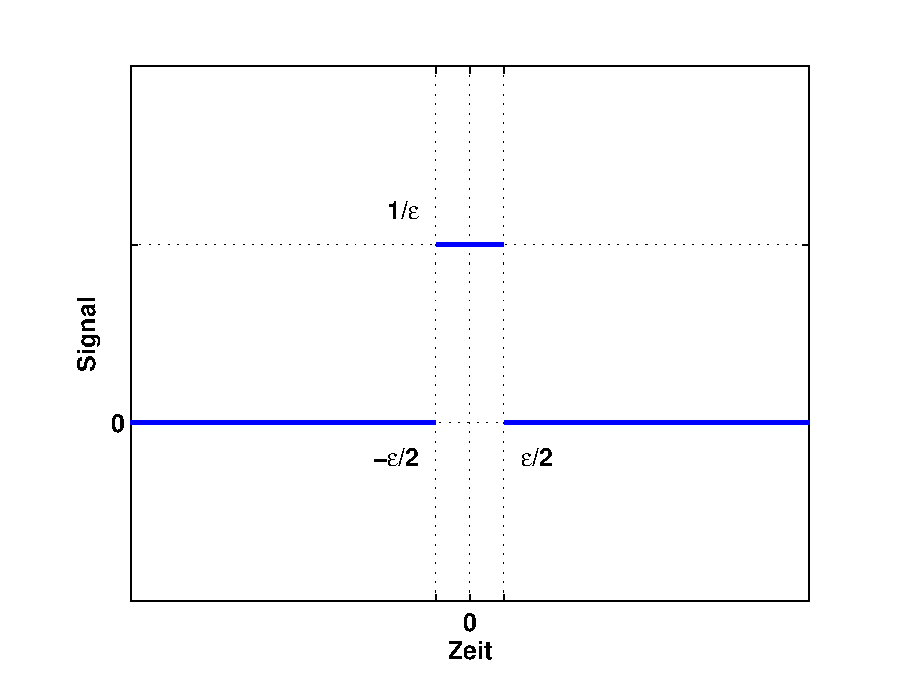
\includegraphics[width=0.5\textwidth]{Kapitel1/Bilder/image11}}
  \caption{Rechteckfunktion mit endlicher Breite $\varepsilon$ zur Ann\"{a}herung der Impulsfunktion}
  \label{fig:NaehrungImpulsfunktion}
\end{figure}

\noindent Mit kleiner werdender Breite $\varepsilon$ wird der das Rechteck immer schmaler, aber auch h\"{o}her, so dass die Fl\"{a}che des Rechtecks immer gleich 1 bleibt. \"{U}ber eine Grenzwertbetrachtung $\varepsilon$ $\rightarrow$ 0 geht diese Rechteckfunktion $\delta$(t) in die Impulsfunktion $\delta$(t) \"{u}ber.

\begin{equation}\label{eq:onethirtysix}
\delta (t)={\lim\limits_{\displaystyle \varepsilon \to 0}} {\rm \; }\left\{\begin{array}{l} 
{0 \qquad \text{ für } \; t<-\varepsilon /2} \\
{1/\varepsilon \quad \, \text{ für } - \varepsilon {\rm /2}<t<\varepsilon /2} \\ 
{0\qquad \text{ für } \; \varepsilon /2{\rm \; }\le {\rm t}} \end{array}\right.
\end{equation}


\noindent Bei der Impulsfunktion $\delta$(t) handelt sich um einen unendlich kurzen Impuls an der Stelle t = 0, der eine unendlich gro{\ss}e H\"{o}he hat. Die Gr\"{o}{\ss}e wird durch einen Pfeil der L\"{a}nge 1 an der Stelle t = 0 dargestellt, weil die Fl\"{a}che unter der Impulsfunktion den Fl\"{a}cheninhalt 1 aufweist. 

\begin{figure}[ht]
  \centerline{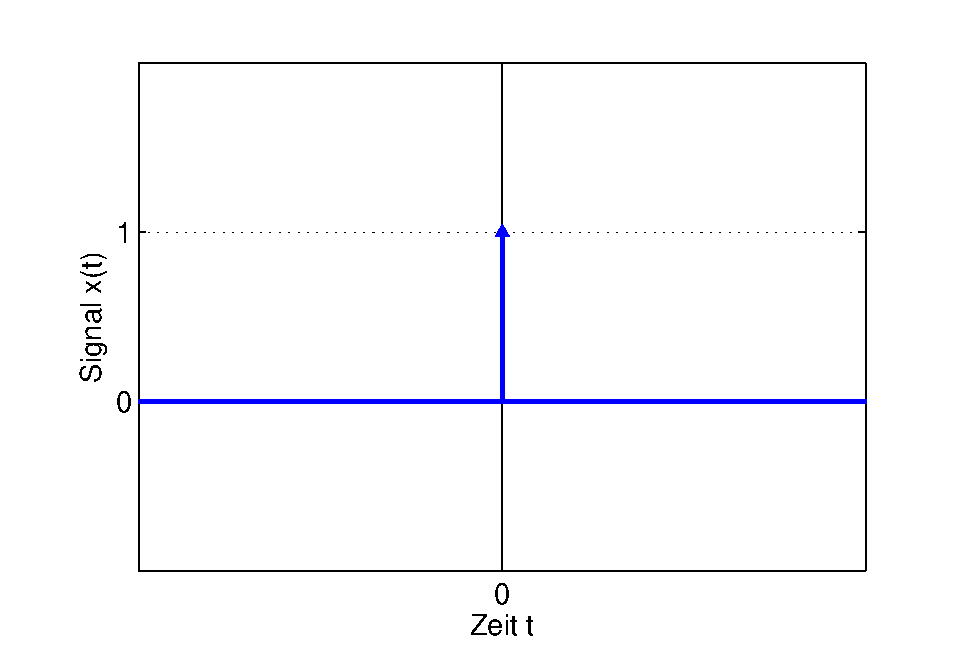
\includegraphics[width=0.5\textwidth]{Kapitel1/Bilder/image12}}
  \caption{Impulsfunktion $\delta$(t)}
  \label{fig:Impulsfunktion}
\end{figure}

\clearpage

\noindent Die Impulsfunktion ist eine gerade Funktion, denn es gilt die Beziehung 

\begin{equation}\label{eq:onethirtyseven}
\delta \left(t\right)=\delta \left(-t\right).
\end{equation}


\noindent Die Impulsfunktion ist eine kausale Funktion, da sie f\"{u}r t $\mathrm{<}$ 0 den Wert null besitzt, und sie ist ein Energiesignal, da sie eine begrenzte Energie besitzt.

\noindent Die Impulsfunktion wird aus Dirac-Impuls bezeichnet und ist als Grenzwert einer gew\"{o}hnlichen Funktion beschrieben. Neben der dargestellten Herleitung \"{u}ber die Rechteckfunktion wird in einem Projekt am Ende dieses Kapitels die Gau{\ss}funktion zur N\"{a}herung des Impulses verwendet. In dem Projekt wird der Impuls anschaulich verglichen mit einem Hammerschlag auf ein schwingungsf\"{a}higes System, zum Beispiel einer Glocke. Das System wird f\"{u}r eine extrem kurze Zeit mit gro{\ss}er Leistung angeregt. Die Glocke antwortet auf die Anregung mit einer Schwingung, die charakteristisch f\"{u}r sie ist. Es wird sich zeigen, dass bestimmte Systeme durch ihre Antwort auf einen Impuls am Eingang vollst\"{a}ndig charakterisiert sind.


\subsubsection{ Rechnen mit Impulsfunktionen}

\noindent Die Impulsfunktion ist Gegenstand der Distributionstheorie [Gelf60]. Hier soll auf Basis der vorgestellten Grenzwertbetrachtung eine anwendungsorientierte Anschauung vermittelt werden, die nicht weiter auf die Distributionstheorie eingeht. Die Gleichung \ref{eq:onethirtyfive} beschreibt den Impuls \"{u}ber eine Rechteckfunktion.

\begin{equation}\label{eq:onethirtyeight}
\delta _{\varepsilon } \left(t\right)=\dfrac{1}{\varepsilon } \cdot \left(\sigma \left(t+\dfrac{\varepsilon }{2} \right)-\sigma \left(t-\dfrac{\varepsilon }{2} \right)\right) \\
\end{equation}
\bigskip

{\fontfamily{phv}\selectfont
\noindent\textbf{Integral der Impulsfunktion}} \smallskip

\noindent Das Integral der Funktion von t = - $\infty$ bis + $\infty$ berechnet sich zu

\begin{equation}\label{eq:onethirtynine}
\int\limits _{-\infty }^{\infty }\delta \left(t\right) \; dt ={\mathop{\lim }\limits_{\varepsilon \to 0}} \; \int\limits _{-\varepsilon /2}^{\varepsilon /2}1/\varepsilon \; dt ={\mathop{\lim }\limits_{\varepsilon \to 0}} \; \dfrac{1}{\varepsilon } \cdot \left(\dfrac{\varepsilon }{2} -\left(-\dfrac{\varepsilon }{2} \right)\right)=\left(\dfrac{\varepsilon }{2\cdot \varepsilon } -\left(-\dfrac{\varepsilon }{2\cdot \varepsilon } \right)\right)=1
\end{equation}


\noindent Das Integral über die Impulsfunktion ist demnach 1. Das Integral der Impulsfunktion wird als Gewicht der Impulsfunktion bezeichnet und wie in Bild \ref{fig:Impulsfunktion} mit einem Pfeil der Länge 1 dargestellt. \bigskip

{\fontfamily{phv}\selectfont
\noindent\textbf{Stammfunktion der Impulsfunktion}} \smallskip

\noindent Die Stammfunktion der Impulsfunktion wird \"{u}ber die N\"{a}herung f\"{u}r die Impulsfunktion bestimmt. Sie ergibt sich mit der Rechteckfunktion $\delta$(t) aus

\begin{equation}\label{eq:onefourty}
\int\limits _{-\infty }^{t}\delta _{\varepsilon } \left(\tau \right) \; d\tau  =\left\{\begin{array}{ll}
{0\qquad \qquad \text{ für } t<-\varepsilon /2} \\
{\dfrac{1}{\varepsilon } \cdot t+\dfrac{ 1}{ 2} \quad \text{ für } -\varepsilon /2<t<\varepsilon /2} \\ 
{1\qquad \qquad  \text{ für }\varepsilon /2 \le t} \end{array}\right. \\
\end{equation}

\noindent Diese Funktion ist die in Bild 2.6 dargestellte verallgemeinerte Sprungfunktion $\sigma$(t). F\"{u}r die hier vorgestellte Grenzwertbetrachtung ergibt sich f\"{u}r die Ableitung der verallgemeinerten Sprungfunktion $\sigma$(t)

\begin{equation}\label{eq:onefourtyone}
\dfrac{d\sigma _{\varepsilon } }{dt} =\left. \left\{\begin{array}{l} 
{0 \qquad \; \text{ für } t<-\varepsilon /2} \\
{\dfrac{1}{\varepsilon} \qquad \text{ für } - \varepsilon /2 <t< \varepsilon /2} \\ 
{0 \qquad \; \text{ für } \varepsilon /2 \le t} \end{array}\right. \right\}=\delta _{\varepsilon } \left(t\right)\\
\end{equation}


\noindent F\"{u}r den Grenzwert $\varepsilon$ $\rightarrow$ 0 ergibt sich die Ableitung der Sprungfunktion

\begin{equation}\label{eq:onefourtytwo}
\dfrac{d\sigma }{dt} =\delta \left(t\right)
\end{equation}


\noindent und umgekehrt die Stammfunktion der Impulsfunktion

\begin{equation}\label{eq:onefourtythree}
\int\limits _{-\infty }^{t}\delta \left(\tau \right){\rm \; }d\tau  =\sigma \left(t\right)
\end{equation}

\bigskip

{\fontfamily{phv}\selectfont
\noindent\textbf{Ausblendeigenschaft der Impulsfunktion}} \smallskip

\noindent Aus der Auswertung des folgenden Integrals ergibt sich eine weitere wichtige Eigenschaft der Impulsfunktion, n\"{a}mlich die Ausblendeigenschaft der Impulsfunktion. Ausgangspunkt ist die Gleichung 

\begin{equation}\label{eq:onefourtyfour}
\int\limits _{-\infty }^{\infty }\delta (t)\cdot x(t) \: dt ={\lim \limits_{\displaystyle\varepsilon \to 0}} \; \dfrac{1}{\varepsilon } \cdot \int\limits _{-\varepsilon /2}^{\varepsilon /2}x(t) \: dt
\end{equation}

\noindent Nach dem Mittelwertsatz der Integralrechnung gibt es ein $t_{0}$ mit $a < t_{0} < b$, f\"{u}r das gilt:

\begin{equation}\label{eq:onefourtyfive}
\int\limits _{a}^{b}x(t) \; dt =(b-a)\cdot x(t_{0} )
\end{equation}

\noindent Damit ergibt sich f\"{u}r Gleichung \ref{eq:onefourtyfour}

\begin{equation}\label{eq:onefourtysix}
\int\limits _{-\infty }^{\infty }\delta (t)\cdot x(t) \; dt ={\lim \limits_{\varepsilon \to 0}} {\rm \; }\dfrac{1}{\varepsilon } \cdot \int\limits _{-\varepsilon /2}^{\varepsilon /2}x(t) \; dt =x(0)
\end{equation}

\noindent Mit dieser Rechenvorschrift l\"{a}sst sich der Abtastwert der Funktion x(t) zum Zeitpunkt t = 0 beschreiben. Die Methode kann f\"{u}r beliebige Zeitpunkte t${}_{0}$ verallgemeinert werden zu

\begin{equation}\label{eq:onefourtyseven}
\int\limits _{-\infty }^{\infty }\delta \left(t-t_{0} \right)\cdot x\left(t\right)\;dt =\int\limits _{-\infty }^{\infty }\delta \left(t\right)\cdot x\left(t+t_{0} \right)\;dt =x\left(t_{0} \right)
\end{equation}

\noindent Die Ausblendeigenschaft der Impulsfunktion wird in Bild \ref{fig:twoAusblendeigenschaftImpulsfunktion} grafisch veranschaulicht. 

\begin{figure}[H]
  \centerline{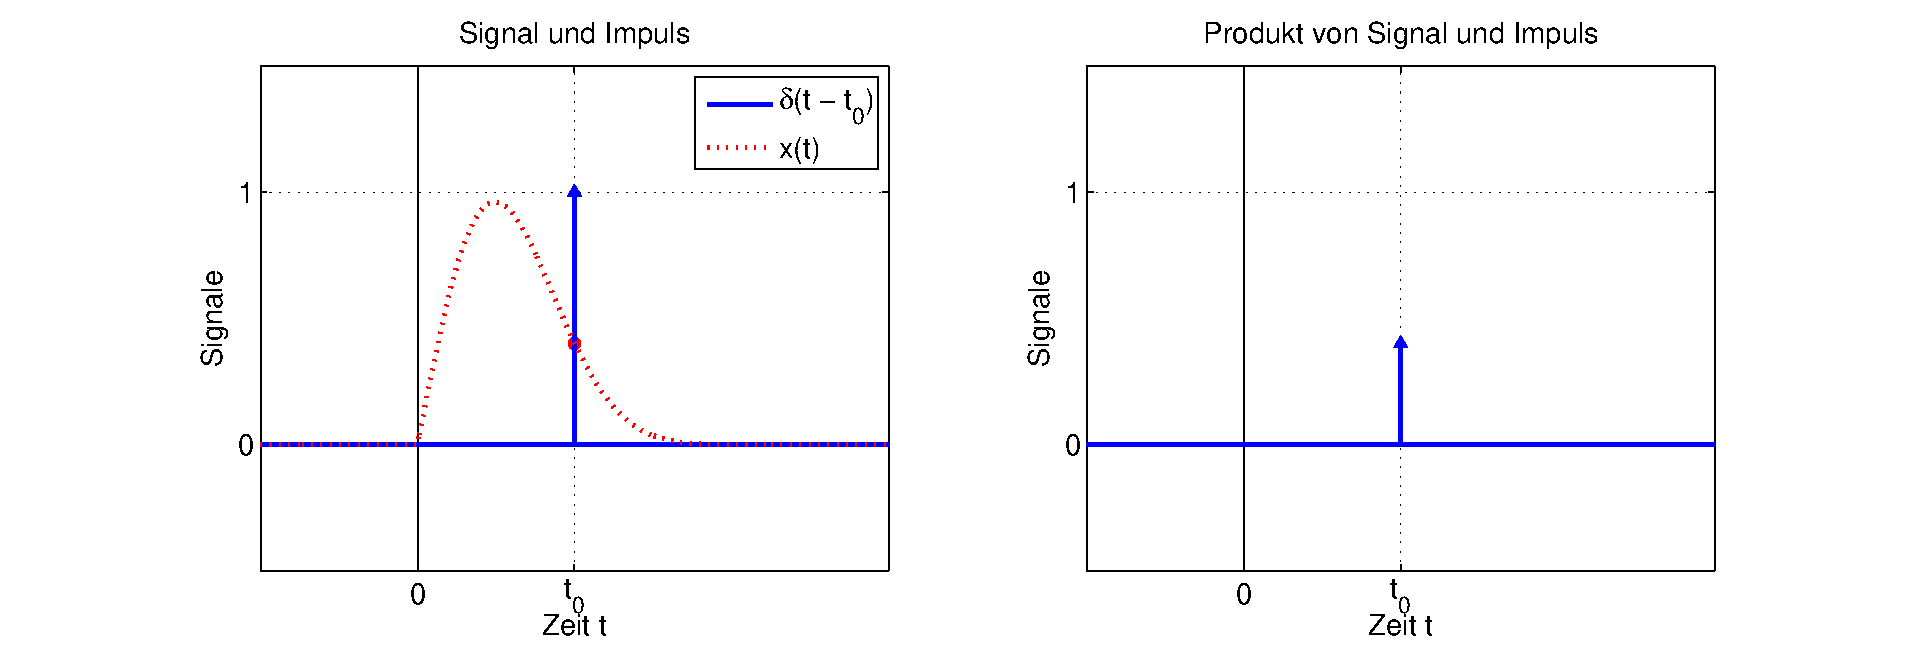
\includegraphics[width=1\textwidth]{Kapitel1/Bilder/image13}}
  \caption{Grafische Darstellung der Ausblendeigenschaft}
  \label{fig:twoAusblendeigenschaftImpulsfunktion}
\end{figure}

\noindent 

\noindent Die Funktion x(t) und die Impulsfunktion an der Stelle t${}_{0}$ sind im Bild links dargestellt. Beide Funktionen werden miteinander multipliziert, das Produkt besteht aus einem Impuls an der Stelle t${}_{0}$ mit dem Gewicht x(t${}_{0}$). Er wird im rechten Bildteil gezeigt. Da das Gewicht des Impulses eine Konstante ist, kann sie aus dem Integral gezogen werden. \"{U}brig bleibt das Integral \"{u}ber eine Impulsfunktion, das nach den diskutierten Rechenregeln den Wert eins aufweist.
\bigskip

{\fontfamily{phv}\selectfont
\noindent\textbf{Ableitung der Impulsfunktion}} \smallskip

\noindent Die Ableitung der Impulsfunktion ist nur bei der Auswertung von Integralen von Bedeutung. In diesem Fall kann die Ableitung durch Anwendung der partiellen Integration umgangen werden.

\begin{equation}\label{eq:onefourtyeight}
\int\limits _{-\infty }^{\infty }\dfrac{d\delta }{dt} \cdot x(t) dt = \delta (t) \cdot x(t)|_{-\infty }^{\infty } -\int\limits _{-\infty }^{\infty }\delta (t)\cdot \dfrac{dx}{dt} dt =-\int\limits _{-\infty }^{\infty }\delta (t)\cdot \dfrac{dx}{dt} dt = -\left. \dfrac{dx}{dt} \right|_{t=0}
\end{equation}

\bigskip

{\fontfamily{phv}\selectfont
\noindent\textbf{Zeitliche Skalierung}} \smallskip

\noindent Wird die Impulsfunktion skaliert, ergibt sich die Funktion

\begin{equation}\label{eq:onefourtynine}
x(t)=\delta (a\cdot t)
\end{equation}


\noindent Mit a $\mathrm{>}$ 0 errechnet sich das Integral in Gleichung \ref{eq:onefourtynine} nach Substitution zu

\begin{equation}\label{eq:fifty}
\int\limits _{-\infty }^{\infty }\delta (a\cdot t) \: dt =\dfrac{1}{a} \cdot \int\limits _{-\infty }^{\infty }\delta (a\cdot t) \: d(a\cdot t) =\dfrac{1}{a}
\end{equation}


\noindent 

\noindent F\"{u}r negative Werte a muss zus\"{a}tzlich die Integrationsreihenfolge ge\"{a}ndert werden, und es ergibt sich ein negatives Vorzeichen. Allgemein gilt 

\begin{equation}\label{eq:onefiftyone}
\int\limits _{-\infty }^{\infty }\delta (a\cdot t) dt =\dfrac{1}{|a|}
\end{equation}


\noindent Eine mit a skalierte Impulsfunktion weist demnach das Gewicht 1/{\textbar}a{\textbar} auf.

\clearpage

\subsubsection{ Zusammenfassung Testfunktionen}

\noindent In Tabelle \ref{tab:twotwo} sind die wesentlichen Testfunktionen und in Tabelle \ref{tab:twothree} die Eigenschaften der Impulsfunktion zusammengefasst.\\


\begin{table}[H]
\setlength{\arrayrulewidth}{.1em}
\caption{Tabellarische Zusammenfassung von Testfunktionen}
\setlength{\fboxsep}{0pt}%
\colorbox{lightgray}{%
\arrayrulecolor{white}%
\begin{tabular}{| l | l |}
\hline
\parbox[c][0.28in][c]{3.3in}{\smallskip\centering\textbf{\fontfamily{phv}\selectfont{Testfunktion}}} & \parbox[c][0.28in][c]{3.3in}{\smallskip\centering\textbf{\fontfamily{phv}\selectfont{Mathematische Beschreibung}}}\\ \hline

\parbox[c][0.64in][c]{3.3in}{\centering{\fontfamily{phv}\selectfont{Sprungfunktion}}} & 
\parbox[c][0.64in][c]{3.3in}{\centering{\fontfamily{phv}\selectfont{$x(t)=\sigma (t)=\left\{\begin{array}{ll} 
0 \text{ für } t<0 \\ 
1\text{ für } 0 \le t  
\end{array}\right. $ }}}\\ \hline 

\parbox[c][0.64in][c]{3.3in}{\centering{\fontfamily{phv}\selectfont{Rechteckfunktion der Länge 2$\cdot$T}}} &
\parbox[c][0.64in][c]{3.3in}{\centering{$x\left(t\right)=\sigma \left(t+T\right)-\sigma \left(t-T\right)$}}\\ \hline


\parbox[c][0.64in][c]{3.3in}{\centering{\fontfamily{phv}\selectfont{Signum-Funktion}}} & 
\parbox[c][0.64in][c]{3.3in}{\centering{\fontfamily{phv}\selectfont{$x(t)=0 $ für $ t<0$}}}\\ \hline

\parbox[c][1in][c]{3.3in}{\centering{\fontfamily{phv}\selectfont{Rampenfunktion}}} & 
\parbox[c][1in][c]{3.3in}{\centering{\fontfamily{phv}\selectfont{$x(t)=\int\limits _{-\infty }^{t}\sigma (\tau )\;d\tau  =t\cdot \sigma (t)=\left\{\begin{array}{ll} 
0 \text{ für } t<0 \\ 
t \text{ für } t \ge 0 
\end{array}\right. $}}}\\ \hline

\parbox[c][0.64in][c]{3.3in}{\centering{\fontfamily{phv}\selectfont{Impulsfunktion}}} & 
\parbox[c][0.64in][c]{3.3in}{\centering{\fontfamily{phv}\selectfont{
$\delta (t)={\mathop{\lim }\limits_{\varepsilon \to 0}} \delta _{\varepsilon } (t)$}}}\\ \hline

\end{tabular}%
}
\label{tab:twotwo}
\end{table}

\bigskip

\begin{table}[H]
\setlength{\arrayrulewidth}{.1em}
\caption{Tabellarische Zusammenfassung der wesentlichen Eigenschaften der Impulsfunktion}
\setlength{\fboxsep}{0pt}%
\colorbox{lightgray}{%
\arrayrulecolor{white}%
\begin{tabular}{| l | l |}
\hline
\parbox[c][0.28in][c]{3.3in}{\smallskip\centering\textbf{\fontfamily{phv}\selectfont{Testfunktion}}} & \parbox[c][0.28in][c]{3.3in}{\smallskip\centering\textbf{\fontfamily{phv}\selectfont{Mathematische Beschreibung}}}\\ \hline

\parbox[c][0.64in][c]{3.3in}{\centering{\fontfamily{phv}\selectfont{Stammfunktion der Impulsfunktion}}} & 
\parbox[c][0.64in][c]{3.3in}{\centering{$x\left(t\right)=\int\limits _{-\infty }^{t}\delta \left(\tau \right) \; d\tau  =\sigma \left(t\right)$ }}\\ \hline 

\parbox[c][1.2in][c]{3.3in}{\centering{\fontfamily{phv}\selectfont{Ausblendeigenschaft der Impulsfunktion}}} & 
\parbox[c][1.2in][c]{3.3in}{\centering{$\int\limits _{-\infty }^{\infty }\delta \left(t-t_{0} \right)\cdot x\left(t\right)\;dt = \qquad \int\limits _{-\infty }^{\infty }\delta \left(t\right)\cdot x\left(t+t_{0} \right)\;dt =x\left(t_{0} \right)$}}\\ \hline


\parbox[c][0.64in][c]{3.3in}{\centering{\fontfamily{phv}\selectfont{Integral über die Impulsfunktion}}} & 
\parbox[c][0.64in][c]{3.3in}{\centering{$\int\limits _{-\infty }^{\infty }\delta \left(t\right)\;dt =1$}}\\ \hline

\parbox[c][0.64in][c]{3.3in}{\centering{\fontfamily{phv}\selectfont}} &
\parbox[c][0.64in][c]{3.3in}{\centering{$\int\limits _{-\infty }^{\infty }\delta \left(a\cdot t\right) \; dt =\dfrac{1}{\left|a\right|} $}}\\ \hline

\end{tabular}%
}
\label{tab:twothree}
\end{table}

\clearpage


\subsection{ Funktionsalgebra}

\noindent Die Berechnung des Ausgangssignals eines linearen Systems kann auf bekannte Ausgangssignale zur\"{u}ckgef\"{u}hrt werden, wenn sich das Eingangssignal auf die entsprechenden Eingangssignale zur\"{u}ckf\"{u}hren l\"{a}sst. Dieses Prinzip wird in Abschnitt \ref{threethreefive} als Superpositionsprinzip eingef\"{u}hrt. Zur Anwendung des Superpositionsprinzips ist es notwendig, Signale mithilfe der in diesem Abschnitt dargestellten Funktionsalgebra umrechnen zu k\"{o}nnen. 


\subsubsection{ Operationen mit kontinuierlichen Funktionen}

\noindent F\"{u}r die Umrechnung von Signalen sind mathematische Operationen notwendig. Die wichtigsten elementaren Operationen sind im Folgenden zusammengefasst. 

\bigskip

{\fontfamily{phv}\selectfont
\noindent\textbf{Skalierung der Amplitude}} \smallskip

\noindent Das Signal a$\cdot$x(t) ist gegen\"{u}ber dem Signal x(t) verst\"{a}rkt (a $\mathrm{>}$ 1) beziehungsweise ged\"{a}mpft (0 $\mathrm{<}$ a $\mathrm{<}$ 1). Bild \ref{fig:Skalierung} zeigt ein Signal x(t) und das um einen Faktor 2 verst\"{a}rkte Signal 2$\cdot$x(t).

\begin{figure}[H]
  \centerline{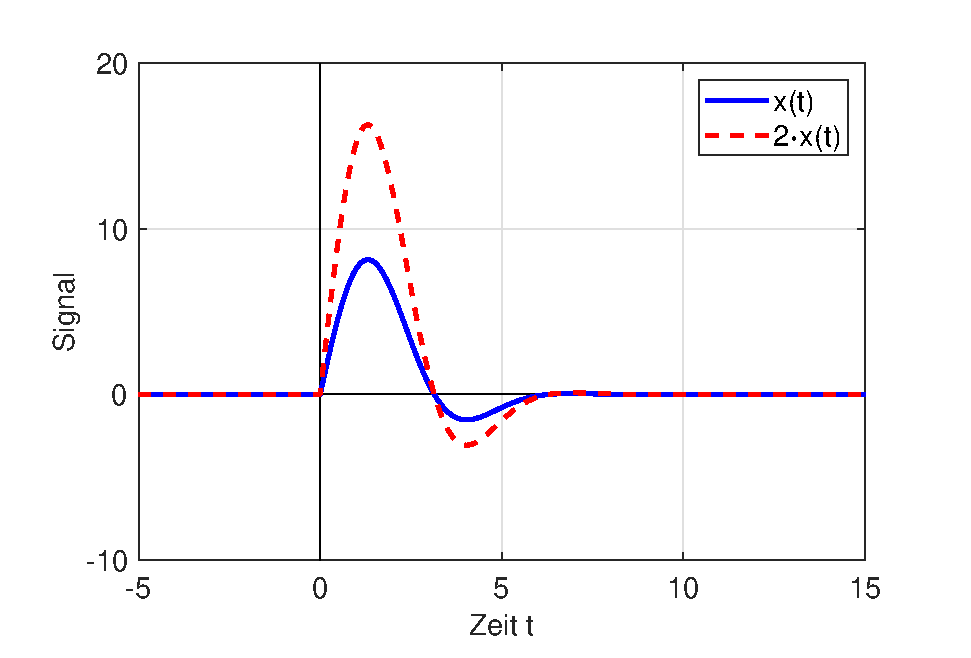
\includegraphics[width=0.5\textwidth]{Kapitel1/Bilder/image14}}
  \caption{Darstellung eines Signals x(t) und eines verst\"{a}rkten Signals 2$\cdot$ x(t)}
  \label{fig:Skalierung}
\end{figure}

\bigskip

{\fontfamily{phv}\selectfont
\noindent\textbf{Zeitliche Verschiebung}} \smallskip

\noindent Das Signal x(t - t${}_{0}$) ist gegen\"{u}ber dem Signal x(t) nach rechts (t${}_{0}$ $\mathrm{>}$ 0) beziehungsweise nach links (t${}_{0}$ $\mathrm{<}$ 0) verschoben. Bild \ref{fig:Verschiebung} zeigt ein Signal x(t) und ein um t${}_{0}$ = 5 nach rechts verschobenes Signal x(t - 5).

\begin{figure}[H]
  \centerline{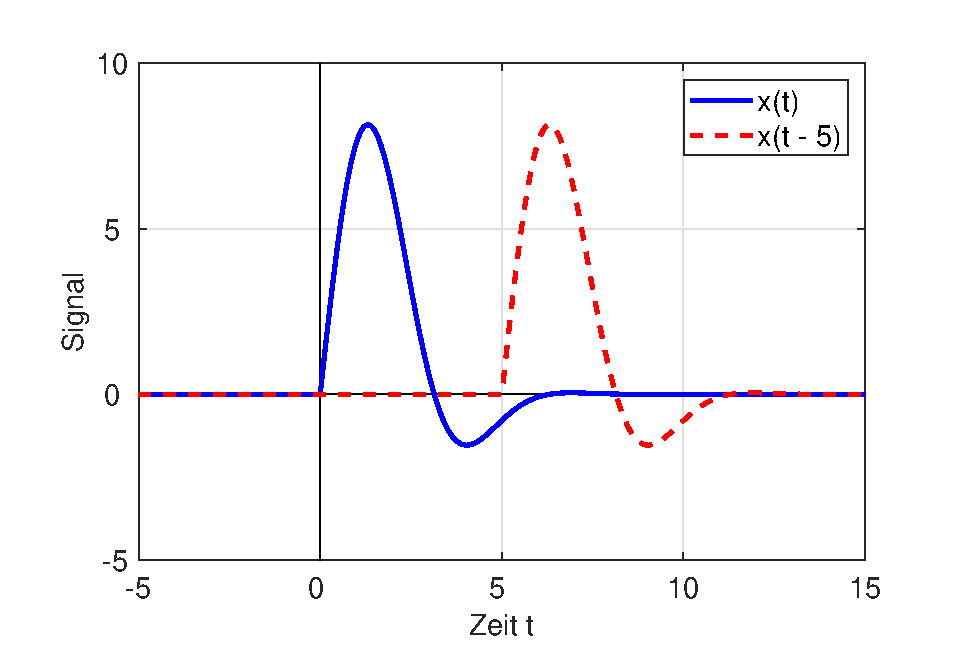
\includegraphics[width=0.5\textwidth]{Kapitel1/Bilder/image15}}
  \caption{Darstellung eines Signals x(t) und des um t${}_{0}$ = 5 nach rechts verschobenen Signals x(t - 5)}
  \label{fig:Verschiebung}
\end{figure}

\clearpage

\noindent Das Vorgehen wird am einfachsten deutlich, wenn das Argument der Funktion analysiert wird. Die Funktion x(t) weist zum Zeitpunkt t = 3 den Funktionswert 0 auf. Da in dem Zeitargument der Funktion x(t - 5) das Argument um 5 verringert wird, weist die Funktion x(t - 5) erst an der Stelle t = 8 den entsprechenden Funktionswert auf.
\bigskip

{\fontfamily{phv}\selectfont
\noindent\textbf{Zeitliche Spiegelung}} \smallskip

\noindent Die Spiegelung eines Signals x(t) an der Stelle t = 0 kann mathematisch durch den Ausdruck x(- t) dargestellt werden. Bild \ref{fig:Spiegelung} zeigt ein Signal x(t) und das gespiegelte Signal x(- t).

\begin{figure}[H]
  \centerline{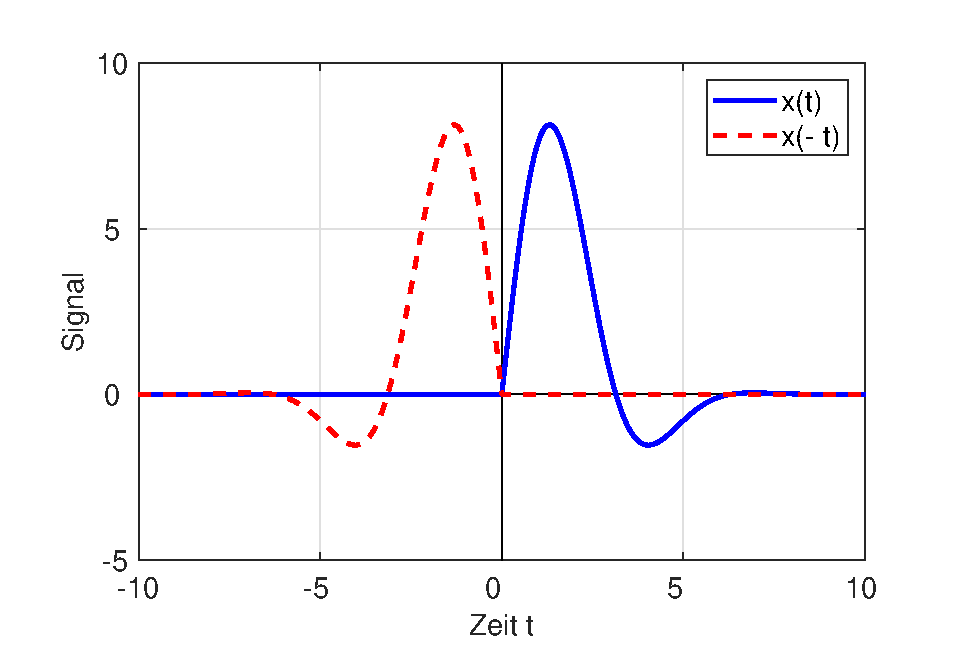
\includegraphics[width=0.5\textwidth]{Kapitel1/Bilder/image16}}
  \caption{Darstellung eines Signals x(t) und des an t = 0 gespiegelten Signals x(t)}
  \label{fig:Spiegelung}
\end{figure}

\noindent Auch hier kann das Zeitargument der Funktion analysiert werden. Die Funktion x(t) weist zum Zeitpunkt t = 1 den Funktionswert 8 auf. Die Funktion x(- t) besitzt denselben Funktionswert an der Stelle t = - 1. 

\bigskip

{\fontfamily{phv}\selectfont
\noindent\textbf{Zeitliche Skalierung}} \smallskip

\noindent Das Signal $x(a.t)$ ist gegenüber dem Signal $x(t)$ gestaucht ($a \mathrm{>} 1$) beziehungsweise gedehnt ($0 \mathrm{<} a \mathrm{<} 1$). Bild \ref{fig:Stauchung} zeigt ein Signal $x(t)$ und ein Signal $x(2.t)$.

\begin{figure}[H]
  \centerline{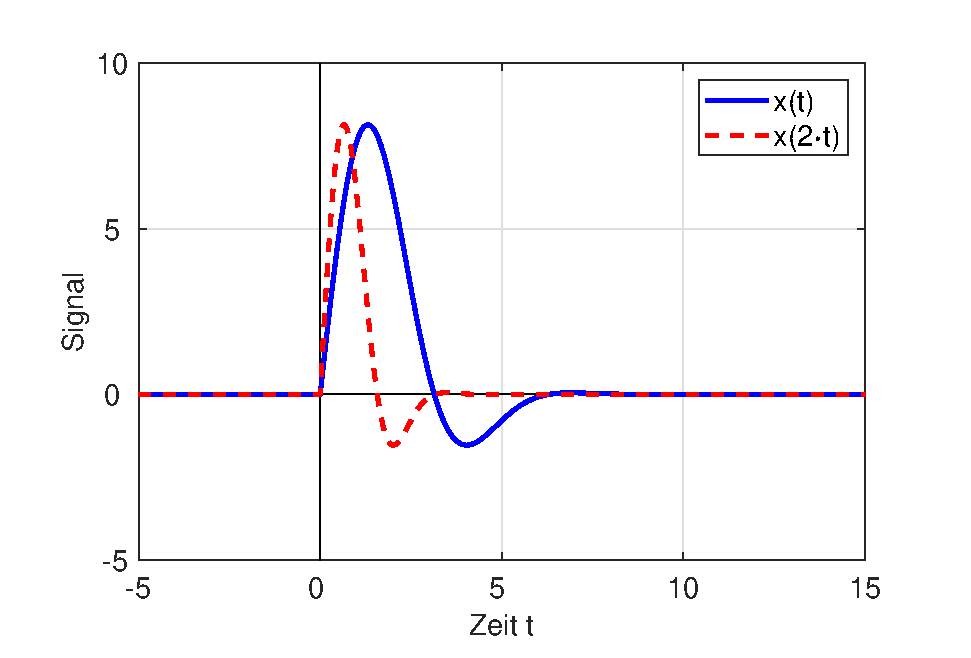
\includegraphics[width=0.5\textwidth]{Kapitel1/Bilder/image17}}
  \caption{Darstellung eines Signals x(t) und eines gestauchten Signals x(2$.$t)}
  \label{fig:Stauchung}
\end{figure}

\noindent Auch Stauchung und Dehnung werden am einfachsten deutlich, wenn das Zeitargument der Funktion x(a$.$t) analysiert wird.

\clearpage

\subsubsection{ Darstellung abschnittsweise definierter Funktionen mit Sprungfunktionen}

\noindent Die vorgestellten Sprung- und Impulsfunktionen erm\"{o}glichen in Kombination mit den vorgestellten Rechenregeln die Synthese weiterer Testfunktionen. An einem Beispiel wird das Rechnen mit Sprungfunktionen verdeutlicht. Das Signal aus Bild \ref{fig:Ueberlagerung} soll durch eine Kombination von Sprungfunktionen geschlossen also ohne Fallunterscheidung dargestellt werden.

\begin{figure}[ht]
  \centerline{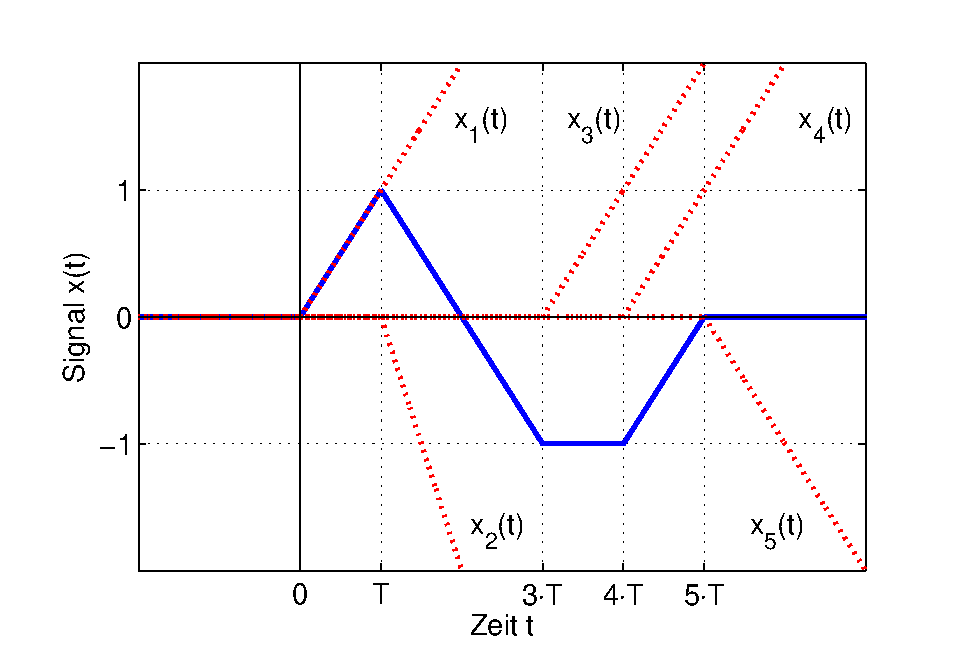
\includegraphics[width=0.5\textwidth]{Kapitel1/Bilder/image18}}
  \caption{Darstellung eines Signals x(t) als Summe von Funktionen}
  \label{fig:Ueberlagerung}
\end{figure}

\noindent Bei der Beschreibung des Signals x(t) sind insbesondere die Stellen von Bedeutung, an denen sich die Steigung des Signals \"{a}ndert. Aus Bild \ref{fig:Ueberlagerung} kann abgelesen werden, dass das die Stellen 0, T, 3$.$T, 4$.$T und 5$.$T sind.

\noindent Zum Zeitpunkt t = 0 beginnt die Funktion, mit einer Steigung 1/T zu steigen. Die Funktion x${}_{1}$(t), die dieses Verhalten beschreibt, ist die Rampenfunktion

\begin{equation}\label{eq:onefiftytwo}
x_{1} \left(t\right)=\dfrac{1}{T} \cdot t\cdot \sigma \left(t\right)
\end{equation}


\noindent Zum Zeitpunkt t = T \"{a}ndert sich die Steigung der Funktion um - 2/T. Der Faktor 2 ergibt sich dabei aus der Kompensation der vor diesem Zeitpunkt vorhandenen Steigung + 1/T und der nach dem Zeitpunkt gew\"{u}nschten Steigung - 1/T. Zu der Funktion x${}_{1}$(t) muss die Funktion x${}_{2}$(t) addiert werden, die aber erst ab dem Zeitpunkt t = T einen Einfluss haben darf. Um die Funktion f\"{u}r t $\mathrm{<}$ T auszublenden, wird die Sprungfunktion verwendet. 

\begin{equation}\label{eq:onefiftythree}
x_{2} \left(t\right)=-\dfrac{2}{T} \cdot \left(t-T\right)\cdot \sigma \left(t-T\right)
\end{equation}

\noindent Das Vorgehen wiederholt sich mit unterschiedlichen Steigungs\"{a}nderungen zu den Zeitpunkten 3$.$T, 4$.$T und 5$.$T, und es ergeben sich die Funktionen 

\begin{equation}\label{eq:onefiftyfour}
x_{3} \left(t\right)=\dfrac{1}{T} \cdot \left(t-3\cdot T\right)\cdot \sigma \left(t-3\cdot T\right)
\end{equation}

\begin{equation}\label{eq:onefiftyfive}
x_{4} \left(t\right)=\dfrac{1}{T} \cdot \left(t-4\cdot T\right)\cdot \sigma \left(t-4\cdot T\right)
\end{equation}


\begin{equation}\label{eq:onefiftysix}
x_{5} \left(t\right)=-\dfrac{1}{T} \cdot \left(t-5\cdot T\right)\cdot \sigma \left(t-5\cdot T\right)
\end{equation}

\noindent Das Signal x(t) kann damit als \"{U}berlagerung der Teilfunktionen x${}_{1}$(t) bis x${}_{5}$(t) dargestellt werden.


\begin{equation}\label{eq:onefiftyseven}
\begin{split}
x(t) & = \dfrac{t}{T} \cdot \sigma \left(t\right)-2\cdot \dfrac{t-T}{T} \cdot \sigma \left(t-T\right)+\dfrac{t-3\cdot T}{T} \cdot \sigma \left(t-3\cdot T\right) \\
 & +\dfrac{t-4\cdot T}{T} \cdot \sigma \left(t-4\cdot T\right)-\dfrac{t-5\cdot T}{T} \cdot \sigma \left(t-5\cdot T\right)
\end{split}
\end{equation}


\noindent Durch den Einsatz der Sprungfunktionen ist gew\"{a}hrleistet, dass die Funktion erst ab einem definierten Zeitpunkt wirkt. Sprungfunktionen erm\"{o}glichen damit die sukzessive Synthese des Signals x(t). 


\subsubsection{ Verallgemeinerte Ableitung}

\noindent Die klassischen Differentiationsregeln erlauben die Berechnung von Ableitungen f\"{u}r stetige Funktionen. In der Systemtheorie werden aber Testfunktionen eingesetzt, die an einer oder mehreren Stellen Spr\"{u}nge aufweisen k\"{o}nnen. Um auch f\"{u}r diese Funktionen Ableitungen angeben zu k\"{o}nnen, wird ein Vorgehen zur Bestimmung einer verallgemeinerten Ableitung von Funktionen mit Spr\"{u}ngen definiert. Dazu wird die Funktion mit einem Sprung an der Stelle t = t${}_{0}$ in eine stetige Funktion x${}_{S}$(t) und einen idealen Sprung der H\"{o}he $\Delta$x an der Stelle t${}_{0}$ zerlegt.

\begin{figure}[ht]
  \centerline{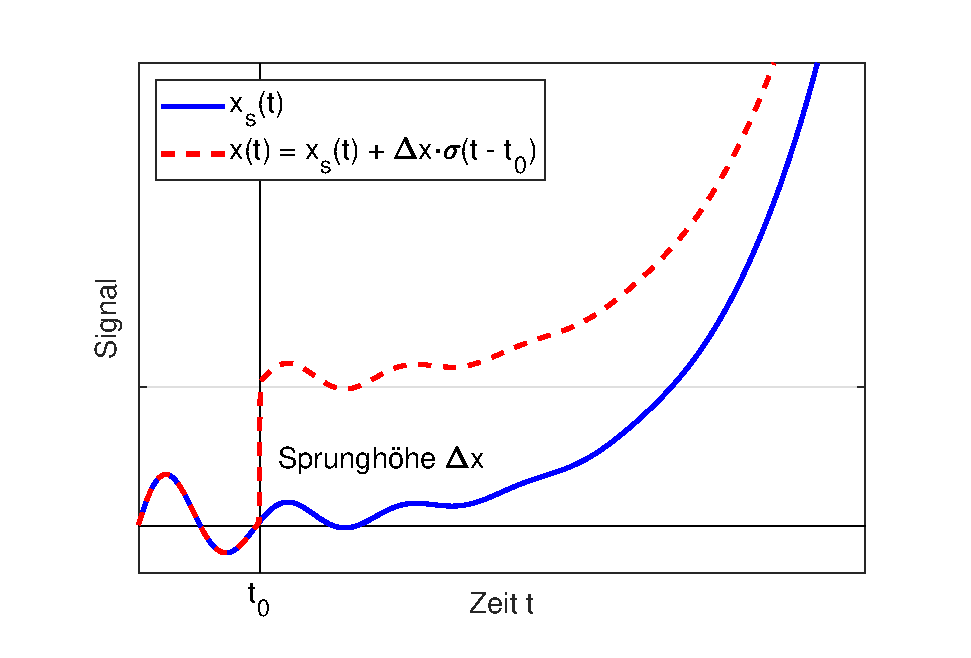
\includegraphics[width=0.5\textwidth]{Kapitel1/Bilder/image19}}
  \caption{Zerlegung der Funktion x(t) in einen stetigen Anteil x${}_{S}$(t) und einen idealen Sprung der H\"{o}he $\Delta$x}
  \label{fig:DifferenzierenErweitert}
\end{figure}
\noindent Die H\"{o}he $\Delta$x des Sprungs ergibt sich aus der Differenz des rechtsseitigen Grenzwertes x(t${}_{0+}$) und linksseitigen Grenzwertes x(t${}_{0-}$) zu 

\begin{equation}\label{eq:onefiftyeight}
\Delta x=x\left(t_{0+} \right)-x\left(t_{0-} \right)
\end{equation}


\noindent Aufgrund der Linearit\"{a}t der Ableitungsoperation und der Ableitung der Sprungfunktion 
\begin{equation}\label{eq:onefiftynine}
\dfrac{d\sigma }{dt} =\delta \left(t\right)
\end{equation}

\noindent errechnet sich die Ableitung der Funktion x(t) zu

\begin{equation}\label{eq:onesixty}
\begin{split}
 \dfrac{dx}{dt}  & =  \dfrac{dx_{S}}{dt} +\dfrac{d}{dt} \left(\sigma \left(t-t_{0} \right)\cdot \left(x\left(t_{0+} \right)-x\left(t_{0-} \right)\right)\right) = \dfrac{dx_{S} }{dt} +\dfrac{d}{dt} \left(\sigma \left(t-t_{0} \right)\cdot \Delta x\right) \\
 & = \dfrac{dx_{S} }{dt} +\delta \left(t-t_{0} \right)\cdot \Delta x 
\end{split}
\end{equation}


\noindent Die verallgemeinerte Ableitung ergibt sich damit aus der Ableitung der stetigen Funktion x${}_{S}$(t) und einem Impuls an der Sprungstelle t${}_{0}$ mit dem Gewicht der Sprungh\"{o}he $\Delta$x. Im Folgenden wird bei der zeitlichen Ableitung immer die verallgemeinerte zeitliche Ableitung angewendet. \clearpage

\noindent
\colorbox{lightgray}{%
\arrayrulecolor{white}%
\renewcommand\arraystretch{0.6}%
\begin{tabular}{ wl{16.5cm} }
{\fontfamily{phv}\selectfont
\noindent{Beispiel: Funktionsalgebra}} 
\end{tabular}%
}\bigskip

\noindent Gegeben ist folgender Signalverlauf x(t). F\"{u}r t $\mathrm{>}$ 6 hat das Signal den Wert null.

\begin{figure}[H]
  \centerline{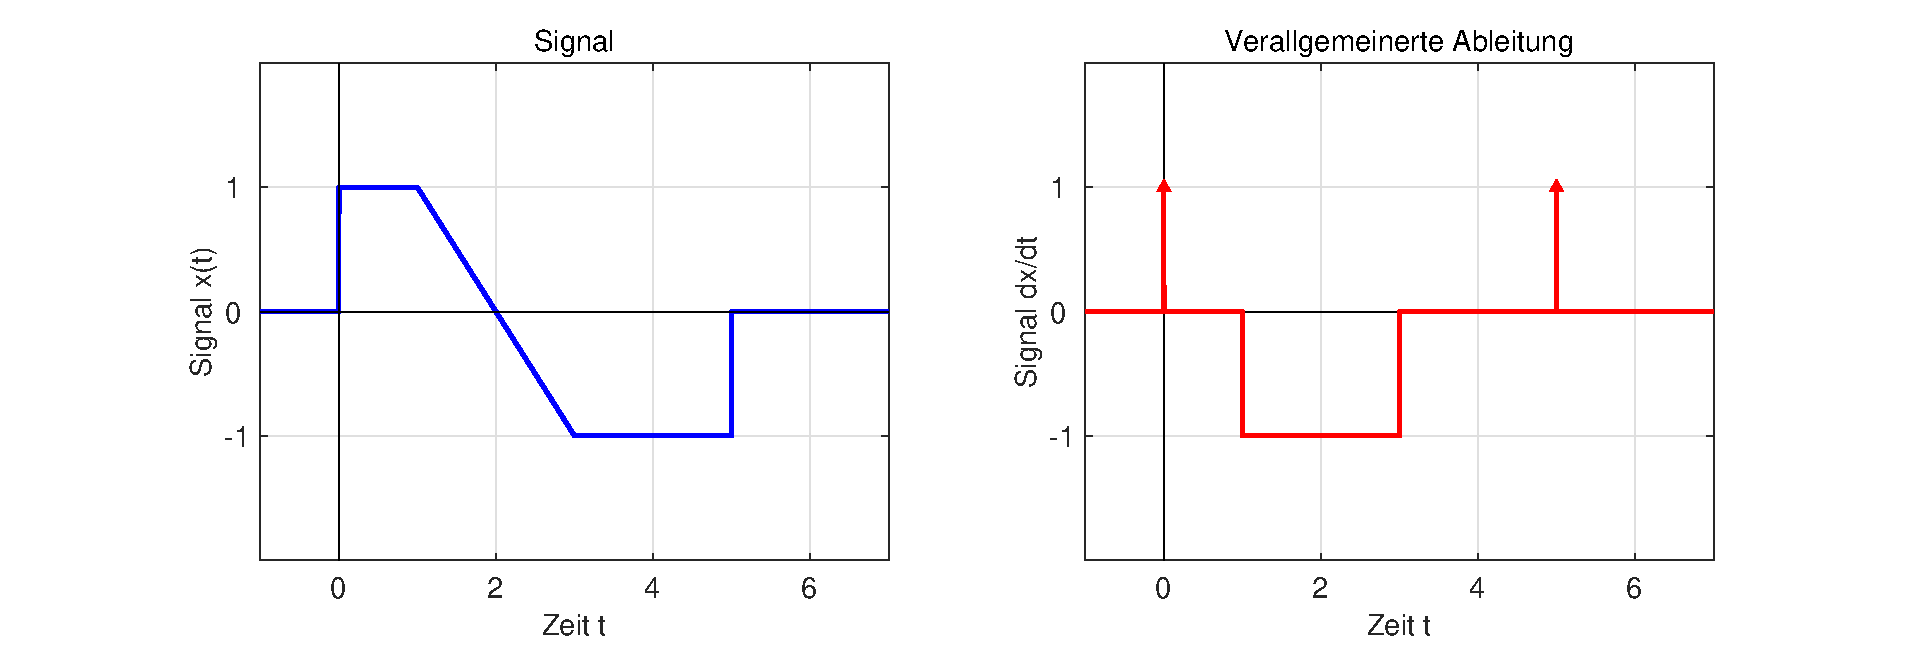
\includegraphics[width=0.8\textwidth]{Kapitel1/Bilder/image20}}
  \caption{Signalverlauf eines Signals x(t) und verallgemeinerte Ableitung des Signalverlaufs}
  \label{fig:BeispielFunktionsalgebra}
\end{figure}

\noindent Das Signal setzt sich aus einem Sprung an der Stelle t = 0, einer Rampe mit negativer Steigung beginnend an der Stelle t = 1 zusammen. Die negative Steigung wird an der Stelle t = 3 kompensiert, an der Stelle t = 5 weist das Signal einen positiven Sprung auf. Mathematisch ergibt sich


\begin{equation}\label{eq:onesixtyone}
x\left(t\right)=\sigma \left(t\right)-\left(t-1\right)\cdot \sigma \left(t-1\right)+\left(t-3\right)\cdot \sigma \left(t-3\right)+\sigma \left(t-5\right)
\end{equation}

\noindent Die Ableitung des Signals erfolgt nach den Rechenregeln der Differentiation mit dem Zusatz der Ableitung von Spr\"{u}ngen. Mit der Produktregel der Differentiation ergibt sich

\begin{equation}\label{eq:onesixtytwo}
\dfrac{dx}{dt} =\delta \left(t\right)-\left(\left(t-1\right)\cdot \delta \left(t-1\right)+\sigma \left(t-1\right)\right)+\left(\left(t-3\right)\cdot \delta \left(t-3\right)+\sigma \left(t-3\right)\right)+\delta \left(t-5\right)
\end{equation}

\noindent In dem Ausdruck treten Terme der Form 

\begin{equation}\label{eq:onesixtythree}
y\left(t\right)=\left(t-t_{0} \right)\cdot \delta \left(t-t_{0} \right)=0
\end{equation}

\noindent auf. Da immer einer der beiden Faktoren null ist, ist das Produkt insgesamt null. Damit kann die Ableitung vereinfacht werden zu 

\begin{equation}\label{eq:onesixtyfour}
\dfrac{dx}{dt} =\delta \left(t\right)-\sigma \left(t-1\right)+\sigma \left(t-3\right)+\delta \left(t-5\right)
\end{equation}

\noindent Die verallgemeinerte Ableitung ist in Bild \ref{fig:BeispielFunktionsalgebra} rechts dargestellt.

\noindent 
\noindent
\noindent


\InsertBoxL{0}{
\includegraphics[scale=0.5]{Code.JPG}} 
\textcolor{white}{.}\newline
\noindent Im Online-Portal \textit{Systemtheorie Online} verdeutlicht die Applikation \textit{Komplexe Exponentialfunktion} den Zusammenhang zwischen der Lage des Wertes $\lambda = \delta + j.\omega{}_{0}$ in der komplexen Ebene und dem Verhalten der Schwingung.\newline


\noindent 


\subsubsection{ Zusammenfassung Funktionsalgebra}

\noindent In Tabelle \ref{tab:twofour} sind die besprochenen Rechenregeln zusammengefasst. Die Anwendung dieser Regeln ist die Zerlegung von Signalen in bekannte Signale. Das Rechnen mit Funktionen ist Grundlage für eine erfolgreiche Anwendung von Korrespondenztafeln der Laplace- und Fourier-Transformation, die in Kapitel 4 und 6 beschrieben werden 

\clearpage

\begin{table}[H]
\setlength{\arrayrulewidth}{.1em}
\caption{Tabellarische Zusammenfassung von Testfunktionen}
\setlength{\fboxsep}{0pt}%
\colorbox{lightgray}{%
\arrayrulecolor{white}%
\begin{tabular}{| l | l |}
\hline
\parbox[c][0.28in][c]{3.3in}{\smallskip\centering\textbf{\fontfamily{phv}\selectfont{Testfunktion}}} & \parbox[c][0.28in][c]{3.3in}{\smallskip\centering\textbf{\fontfamily{phv}\selectfont{Mathematische Beschreibung}}}\\ \hline

\parbox[c][0.64in][c]{3.3in}{\centering{\fontfamily{phv}\selectfont{Skalierung der Amplitude}}} & 
\parbox[c][0.64in][c]{3.3in}{\centering{$y\left(t\right)=a\cdot x\left(t\right)$}}\\ \hline

\parbox[c][0.64in][c]{3.3in}{\centering{\fontfamily{phv}\selectfont{Zeitliche Verschiebung um $t{}_{0}$}}} & \parbox[c][0.64in][c]{3.3in}{\centering{$y\left(t\right)=x\left(t-t_{0} \right)$}}\\ \hline

\parbox[c][0.64in][c]{3.3in}{\centering{\fontfamily{phv}\selectfont{Zeitliche Spiegelung}}} & 
\parbox[c][0.64in][c]{3.3in}{\centering{$y\left(t\right)=x\left(-t\right)$}}\\ \hline

\parbox[c][0.64in][c]{3.3in}{\centering{\fontfamily{phv}\selectfont{Zeitliche Skalierung}}} & 
\parbox[c][0.64in][c]{3.3in}{\centering{$y\left(t\right)=x\left(a\cdot t\right)$}}\\ \hline

\parbox[c][0.64in][c]{3.3in}{\centering{\fontfamily{phv}\selectfont{Verallgemeinerte Ableitung einer Funktion x(t)mit Sprung $\Delta$x an der Stelle $t{}_{0}$}}} &
\parbox[c][0.64in][c]{3.3in}{\centering{$\dfrac{dx}{dt} =\dfrac{dx_{S} }{dt} +\delta \left(t-t_{0} \right)\cdot \Delta x$}}\\ \hline

\end{tabular}%
}
\label{tab:twofour}
\end{table}

\clearpage 


\subsection{ Funktionen zur Beschreibung von Einschwingvorg\"{a}ngen}


\subsubsection{ Periodische und harmonische Funktionen}

Periodische Funktionen sind dadurch gekennzeichnet, dass sich der Funktionswert periodisch nach einer Zeitdauer T${}_{0}$ wiederholt. Bild \ref{fig:Periodisch} zeigt ein einfaches periodisches Signal.

\begin{figure}[ht]
  \centerline{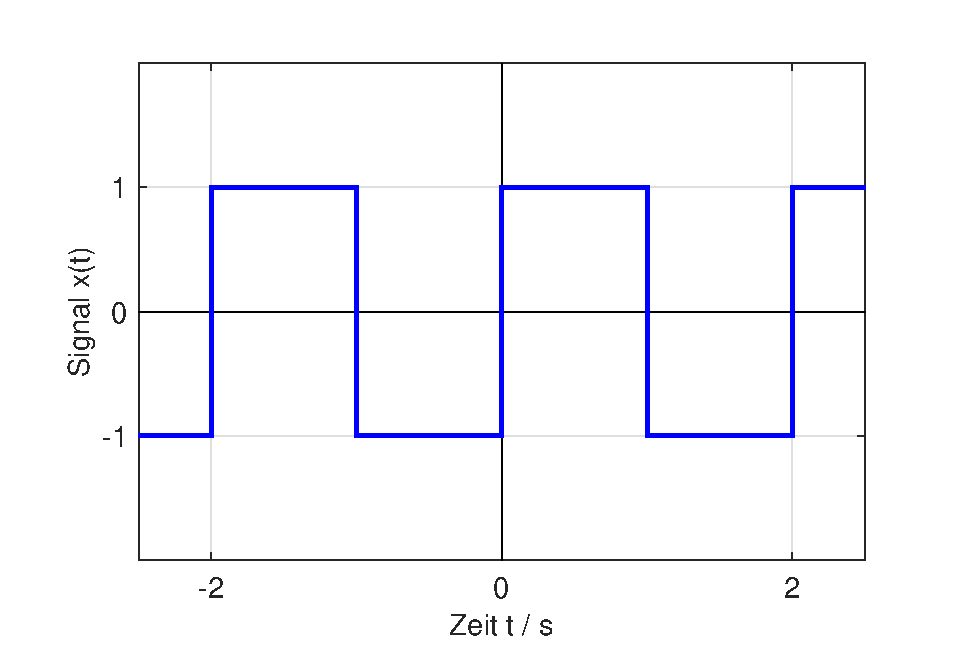
\includegraphics[width=0.5\textwidth]{Kapitel1/Bilder/image21}}
  \caption{Beispiel f\"{u}r ein periodisches Signal mit einer Periodendauer T${}_{0}$ = 2 s }
  \label{fig:Periodisch}
\end{figure}

\noindent F\"{u}r periodische Funktionen und ganzzahlige Werte k gilt:

\begin{equation}\label{eq:onesixtyfive}
x\left(t\right)=x\left(t+k\cdot T_{0} \right)
\end{equation}

\noindent Neben den bereits diskutierten Testfunktionen, die das Ein-, Aus- oder Umschalten modellieren, sind in der Systemtheorie periodische, harmonische Signale von gro{\ss}er Bedeutung. Als Beispiel soll hier eine Kosinusfunktion diskutiert werden. Sie ist definiert als

\begin{equation}\label{eq:onesixtysix}
x\left(t\right)=A\cdot \cos \left(\omega _{0} \cdot t+\varphi \right)=A\cdot \cos \left(\omega _{0} \cdot \left(t+t_{0} \right)\right)
\end{equation}

\noindent mit

\begin{equation}\label{eq:onesixtyseven}
t_{0} =\dfrac{\varphi }{\omega _{0} } 
\end{equation}

\noindent wobei A die Amplitude der Schwingung, $\varphi$ der Nullphasenwinkel und $\omega{}_{0}$ die Kreisfrequenz ist.

\begin{equation}\label{eq:onesixtyeight}
\omega _{0} =\dfrac{2\cdot \pi }{T_{0} } =2\cdot \pi \cdot f_{0} 
\end{equation}

\noindent Die Frequenz f${}_{0}$ der Funktion x(t) ist der Kehrwert der Periodendauer T${}_{0}$ der Schwingung.

\begin{equation}\label{eq:onesixtynine}
f_{0} =\dfrac{1}{T_{0} } =\dfrac{\omega _{0} }{2\cdot \pi }
\end{equation}

\clearpage
\noindent Bild \ref{fig:Inconnue} verdeutlicht diese Definitionen an einem Beispiel:

\begin{figure}[ht]
  \centerline{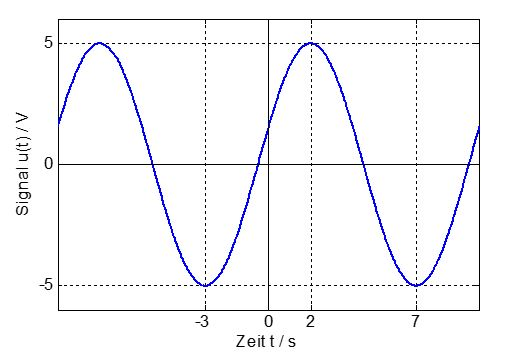
\includegraphics[width=0.5\textwidth]{Kapitel1/Bilder/image22.JPG}}
  \caption{Kosinusfunktion mit einer Periodendauer T${}_{0}$ = 10 s, einer Amplitude von 5 V und einem Nullphasenwinkel von - 2/5$.$$\pi$ }
  \label{fig:Inconnue}
\end{figure}

\noindent In dem Beispiel beträgt die Amplitude 5 V. Die Kosinusfunktion hat zwei aufeinanderfolgende Minima bei t = - 3 s und t = 7 s, woraus sich eine Periodendauer von T${}_{0}$ = 10 s ergibt. Die Nullphase $\varphi$ ist nicht unmittelbar aus dem Diagramm ablesbar. Die Kosinusfunktion ist in Bild 2.22 um 2 s nach rechts verschoben. Es liegt demnach eine zeitliche Verz\"{o}gerung von t${}_{0}$ = - 2 s vor. \"{U}ber den Zusammenhang

\begin{equation}\label{eq:oneseventy}
t_{0} =\dfrac{\varphi }{2\cdot \pi \cdot f_{0} } =\dfrac{\varphi }{2\cdot \pi } \cdot T_{0} =-2 \; s
\end{equation}


\noindent kann der Nullphasenwinkel $\varphi$ berechnet werden zu

\begin{equation}\label{eq:oneseventyone}
\varphi =-\dfrac{2\cdot \pi \cdot 2\;s}{10\;s} =-\dfrac{2\cdot \pi }{5}
\end{equation}

\bigskip

{\fontfamily{phv}\selectfont
\noindent\textbf{\"{U}berlagerung harmonischer Signale}} \smallskip

\noindent Harmonische Signale mit Nullphasenwinkel k\"{o}nnen mithilfe der Additionstheoreme als Summe von einer Sinus- und einer Kosinusfunktion dargestellt werden.

\begin{equation}\label{eq:oneseventytwo}
\sin \left(a+b\right)=\sin \left(a\right)\cdot \cos \left(b\right)+\cos \left(a\right)\cdot \sin \left(b\right)
\end{equation}


\begin{equation}\label{eq:oneseventythree}
\sin \left(a-b\right)=\sin \left(a\right)\cdot \cos \left(b\right)-\cos \left(a\right)\cdot \sin \left(b\right)
\end{equation}


\begin{equation}\label{eq:oneseventyfour}
\cos \left(a+b\right)=\cos \left(a\right)\cdot \cos \left(b\right)-\sin \left(a\right)\cdot \sin \left(b\right)
\end{equation}

\begin{equation}\label{eq:oneseventyfive}
\cos \left(a-b\right)=\cos \left(a\right)\cdot \cos \left(b\right)+\sin \left(a\right)\cdot \sin \left(b\right)
\end{equation}

\noindent Eine Kosinusfunktion mit dem Nullphasenwinkel $\varphi$ kann also als Summe einer Kosinus- und Sinusfunktion mit Nullphasenwinkel $\varphi$ = 0 dargestellt werden.

\begin{equation}\label{eq:oneseventysix}
\begin{split}
x(t) & = A\cdot \cos \left(\omega _{0} \cdot t+\varphi \right) \\ 
 & = A\cdot \cos \left(\omega _{0} \cdot t\right)\cdot \cos \left(\varphi \right)-A\cdot \sin \left(\omega _{0} \cdot t\right)\cdot \sin \left(\varphi \right) \\
 & = a\cdot \cos \left(\omega _{0} \cdot t\right)-b\cdot \sin \left(\omega _{0} \cdot t\right)
\end{split}
\end{equation}

\noindent wobei sich deren Amplituden durch einen Koeffizientenvergleich ergeben zu 

\begin{equation}\label{eq:oneseventyseven}
a=A\cdot \cos \left(\varphi \right)
\end{equation}


\begin{equation}\label{eq:oneseventyeight}
b=A\cdot \sin \left(\varphi \right)
\end{equation}

\noindent Umgekehrt k\"{o}nnen eine Kosinus- und eine Sinusfunktion gleicher Frequenz addiert werden zu einer resultierenden Schwingung mit Amplitude A und Nullphasenwinkel $\varphi$:

\begin{equation}\label{eq:oneseventynine}
\begin{split}
x\left(t\right) & = a\cdot \cos \left(\omega _{0} \cdot t\right)-b\cdot \sin \left(\omega _{0} \cdot t\right) \\ 
& = A\cdot \cos \left(\varphi \right)\cdot \cos \left(\omega _{0} \cdot t\right)-A\cdot \sin \left(\varphi \right)\cdot \sin \left(\omega _{0} \cdot t\right) \\ 
& = A\cdot \cos \left(\omega _{0} \cdot t+\varphi \right)    
\end{split}
\end{equation}


\noindent Dabei ergeben sich Amplitude und Nullphasenwinkel aus 

\begin{equation}\label{eq:oneeighty}
A=\sqrt{a^{2} +b^{2} } 
\end{equation}

\begin{equation}\label{eq:oneeightyone}
\tan \left(\varphi \right)=\dfrac{\sin \left(\varphi \right)}{\cos \left(\varphi \right)} =\dfrac{b}{a} 
\end{equation}

\noindent Aus einer \"{U}berlagerung von Sinus- und Kosinusfunktionen gleicher Frequenz resultiert eine Sinus- oder Kosinusfunktion mit derselben Frequenz, aber unterschiedlicher Amplitude und Nullphase.\bigskip

{\fontfamily{phv}\selectfont
\noindent\textbf{Zeigerdarstellung harmonischer Signalen}} \smallskip

\noindent In der Elektrotechnik hat sich f\"{u}r die Berechnung von harmonisch angeregten Schaltungen die Zeigerdarstellung durchgesetzt. Sie beruht auf der Eulerschen Formel.

\begin{equation}\label{eq:oneeightytwo}
e^{j\cdot \varphi } =\cos \left(\varphi \right)+j\cdot \sin \left(\varphi \right)
\end{equation}


\noindent Damit kann eine Kosinusfunktion der Form

\begin{equation}\label{eq:oneeightythree}
x\left(t\right)=A\cdot \cos \left(\omega _{0} \cdot t+\varphi \right)
\end{equation}


\noindent als Realteil einer komplexen Funktion

\begin{equation}\label{eq:oneeightyfour}
z\left(t\right)=A\cdot e^{j\cdot \left(\omega _{0} \cdot t+\varphi \right)} =A\cdot e^{j\cdot \varphi } \cdot e^{j\cdot \omega _{0} \cdot t} =A\cdot \left(\cos \left(\omega _{0} \cdot t+\varphi \right)+j\cdot \sin \left(\omega _{0} \cdot t+\varphi \right)\right)
\end{equation}


\noindent aufgefasst werden. Diese mathematische Darstellung kann durch einen Zeiger der L\"{a}nge A verdeutlicht werden, der in der komplexen Ebene um den Koordinatenursprung rotiert. Die Zeit f\"{u}r eine volle Umdrehung ist die Periodendauer T${}_{0}$. Die eigentlich interessierende Gr\"{o}{\ss}e ist die Projektion des Zeigers auf die reelle Achse, sie stellt die Funktion x(t) dar. Zum Zeitpunkt t = 0 gilt

\begin{equation}\label{eq:oneeightyfive}
z\left(0\right)=A\cdot e^{j\cdot \varphi } =A\cdot \cos \left(\varphi \right)+j\cdot A\cdot \sin \left(\varphi \right)=\underline{A}
\end{equation}

\noindent \underbar{A} wird als komplexe Amplitude der komplexen Funktion z(t) bezeichnet. Ein Vergleich der Koeffizienten mit Gleichung \ref{eq:oneseventysix} zeigt, dass die komplexe Amplitude \underbar{A} dargestellt werden kann, als 

\begin{equation}\label{eq:oneeightysix}
\underline{A}=a+j\cdot b
\end{equation}


\noindent Zur Verdeutlichung der komplexen Amplitude \underbar{A} zeigt Bild \ref{fig:HarmonischeSchwingung} eine Zeigerdarstellung in der komplexen Ebene. Sie illustriert die Projektion des komplexen Zeigers auf die reelle Achse als Zeitfunktion x(t).

\noindent 
\begin{figure}[H]
  \centerline{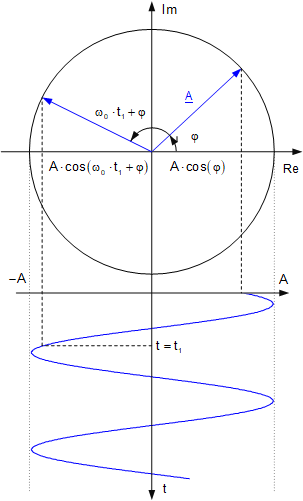
\includegraphics[width=0.45\textwidth]{Kapitel1/Bilder/image23}}
  \caption{Darstellung einer harmonischen Schwingung als Zeigerdiagramm }
  \label{fig:HarmonischeSchwingung}
\end{figure}

\medskip
{\fontfamily{phv}\selectfont
\noindent\textbf{Darstellung harmonischer Signale als Überlagerung komplexer Schwingungen}} \smallskip

\noindent Durch Umformung von Gleichung \ref{eq:oneeightytwo} ergibt sich f\"{u}r Sinus- und Kosinusfunktionen die Darstellung


\begin{equation}\label{eq:oneeightyseven}
\cos \left(\varphi \right)=\dfrac{1}{2} \cdot \left(e^{j\cdot \varphi } +e^{-j\cdot \varphi } \right)
\end{equation}

\begin{equation}\label{eq:oneeightyeight}
\sin \left(\varphi \right)=\dfrac{1}{2\cdot j} \cdot \left(e^{j\cdot \varphi } -e^{-j\cdot \varphi } \right)=-\dfrac{1}{2} \cdot j\cdot \left(e^{j\cdot \varphi } -e^{-j\cdot \varphi } \right)
\end{equation}


\noindent Werden in Gleichung \ref{eq:oneseventynine} die reellen Sinus- und Kosinusfunktionen durch Summen komplexer Funktionen nach Gleichung \ref{eq:oneeightyseven} und \ref{eq:oneeightyeight} ersetzt, so ergibt sich 

\begin{equation}\label{eq:oneeightynine}
\begin{split}
x(t) & = a\cdot \cos \left(\omega _{0} \cdot t\right)-b\cdot \sin \left(\omega _{0} \cdot t\right) \\ 
 & = a\cdot \dfrac{1}{2} \cdot \left(e^{j\cdot \omega _{0} \cdot t} +e^{-j\cdot \omega _{0} \cdot t} \right)-b\cdot \dfrac{1}{2\cdot j} \cdot \left(e^{j\cdot \omega _{0} \cdot t} -e^{-j\cdot \omega _{0} \cdot t} \right) \\ 
 & = \dfrac{1}{2} \cdot \left(a+j\cdot b\right)\cdot e^{j\cdot \omega _{0} \cdot t} +\dfrac{1}{2} \cdot \left(a-j\cdot b\right)\cdot e^{-j\cdot \omega _{0} \cdot t } 
\end{split}
\end{equation}


\noindent Der erste Summand beschreibt einen komplexen Zeiger, der sich in der komplexen Ebene mit einer Periodendauer T${}_{0}$ in mathematisch positiver Richtung dreht. Der zweite Summand beschreibt einen zweiten komplexen Zeiger, der zu jedem Zeitpunkt konjugiert komplex zum Ersten ist. Er dreht sich mit derselben Winkelgeschwindigkeit wie der erste Zeiger, aber in entgegengesetzter Richtung. 

\noindent Aus den komplexen Koeffizienten 

\begin{equation}\label{eq:oneninety}
\underline{c}=\dfrac{a+j\cdot b}{2}
\end{equation}

\begin{equation}\label{eq:oneninetyone}
\underline{c}*=\dfrac{a-j\cdot b}{2}
\end{equation}

\noindent errechnen sich die Amplitude A und der Nullphasenwinkel $\varphi$ zu

\begin{equation}\label{eq:oneninetytwo}
A=2\cdot \left|\underline{c}\right|
\end{equation}

\begin{equation}\label{eq:oneninetythree}
\varphi =\arg \left(\underline{c}\right)
\end{equation}

\noindent Die komplexe Exponentialfunktion stellt reelle Funktionen mithilfe komplexer Zahlen dar. Es ist eine effiziente Beschreibungsform, die gleicherma{\ss}en Amplitude und Phase beschreibt. Physikalisch gesehen existieren komplexe Signale nicht.

\noindent
\noindent

%%%%%%%%%%%%%% CODE BILD

\clearpage


\subsubsection{ Exponentialfunktion}

\noindent Bei der Diskussion von Systemen wird sich zeigen, dass die Exponentialfunktion 

\begin{equation}\label{eq:oneninetyfour}
x\left(t\right)=A\cdot e^{\lambda \cdot t} \cdot \sigma \left(t\right)
\end{equation}

 
\noindent die Einschwingvorgänge vieler physikalischer Vorgänge beschreiben kann. Bild \ref{fig:Exponentialfunktion} stellt das Verhalten der Exponentialfunktion für unterschiedliche reelle Parameter $\lambda$ im Zeitraum t $\mathrm{>}$ 0 dar.

\begin{figure}[ht]
  \centerline{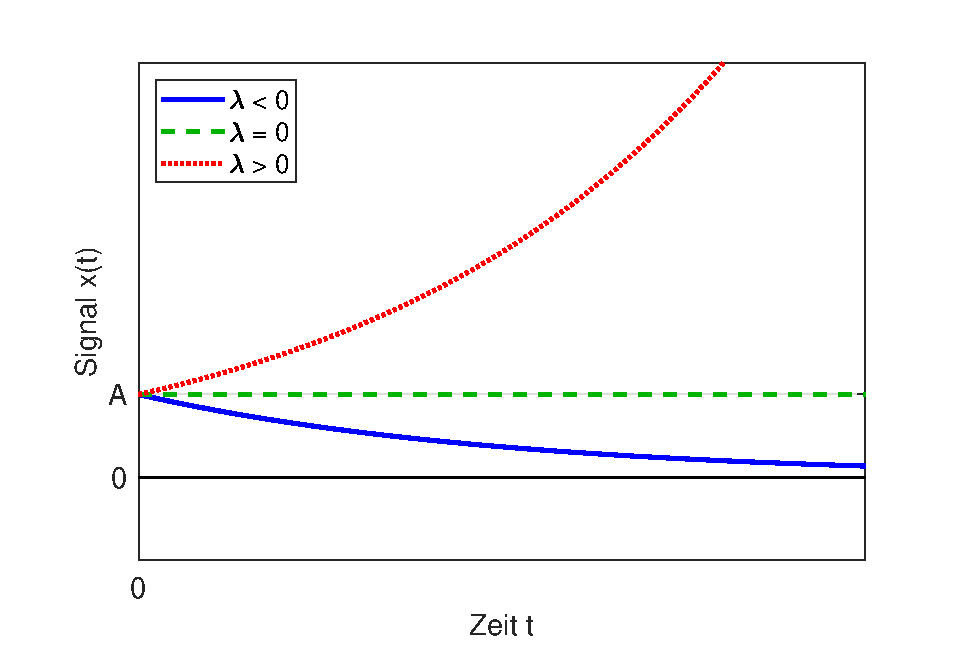
\includegraphics[width=0.5\textwidth]{Kapitel1/Bilder/image24}}
  \caption{Darstellung der Exponentialfunktion f\"{u}r unterschiedliche Parameter $\lambda$ }
  \label{fig:Exponentialfunktion}
\end{figure}

\noindent Die Exponentialfunktion beginnt f\"{u}r alle Parameter $\lambda$ an der Stelle x(t = 0) = A. F\"{u}r reelle Parameter $\lambda$ $\mathrm{>}$ 0 steigt die Exponentialfunktion mit wachsender Zeit t. Bei negativem reellen Parameter $\lambda$ $\mathrm{<}$ 0 n\"{a}hert sich die Exponentialfunktion der Asymptote x = 0. F\"{u}r $\lambda$ = 0 bleibt die Exponentialfunktion konstant bei x = A.

\noindent Im vorangegangenen Abschnitt wird auf Exponentialfunktionen mit rein imagin\"{a}ren Werten von $\lambda$ verwiesen, und es wird aufgezeigt, dass sie harmonische Schwingungen beschreiben k\"{o}nnen. Au{\ss}er reellen und imagin\"{a}ren Argumenten k\"{o}nnen bei Exponentialfunktionen auch komplexe Argumente $\lambda$ auftreten. In diesem Fall kann die Exponentialfunktion in zwei Faktoren zerlegt werden:

\begin{equation}\label{eq:oneninetyfive}
e^{\lambda \cdot t} =e^{\left(\delta _{0} +j\cdot \omega _{0} \right)\cdot t} =e^{\delta _{0} \cdot t} \cdot e^{j\cdot \omega _{0} \cdot t}
\end{equation}

\noindent Damit kann eine Kosinusfunktion mit exponentiell abklingender Amplitude als Summe zweier Exponentialfunktionen mit jeweils konjugiert komplexen Koeffizienten $\lambda$ dargestellt werden. 

\begin{equation}\label{eq:oneninetysix}
\begin{split}
x(t) & ={A\cdot e^{\delta _{0} \cdot t} \cdot \cos \left(\omega _{0} \cdot t\right)\cdot \sigma \left(t\right)=\dfrac{1}{2} \cdot A\cdot e^{\delta _{0} \cdot t} \cdot \left(e^{j\cdot \omega _{0} \cdot t} +e^{-j\cdot \omega _{0} \cdot t} \right)\cdot \sigma \left(t\right)} \\
& = \dfrac{1}{2} \cdot A\cdot \left(e^{\left(\delta _{0} +j\cdot \omega _{0} \right)\cdot t} +e^{\left(\delta _{0} -j\cdot \omega _{0} \right)\cdot t} \right)\cdot \sigma \left(t\right)    
\end{split}
\end{equation}


\noindent Die Kosinusfunktion mit exponentiell abklingender Amplitude ist in Bild \ref{fig:KomplexExponentialfunktion} dargestellt. Dabei sind die Einh\"{u}llenden der Kosinusfunktion als gestrichelte Linie eingezeichnet.

\clearpage
\begin{figure}[H]
  \centerline{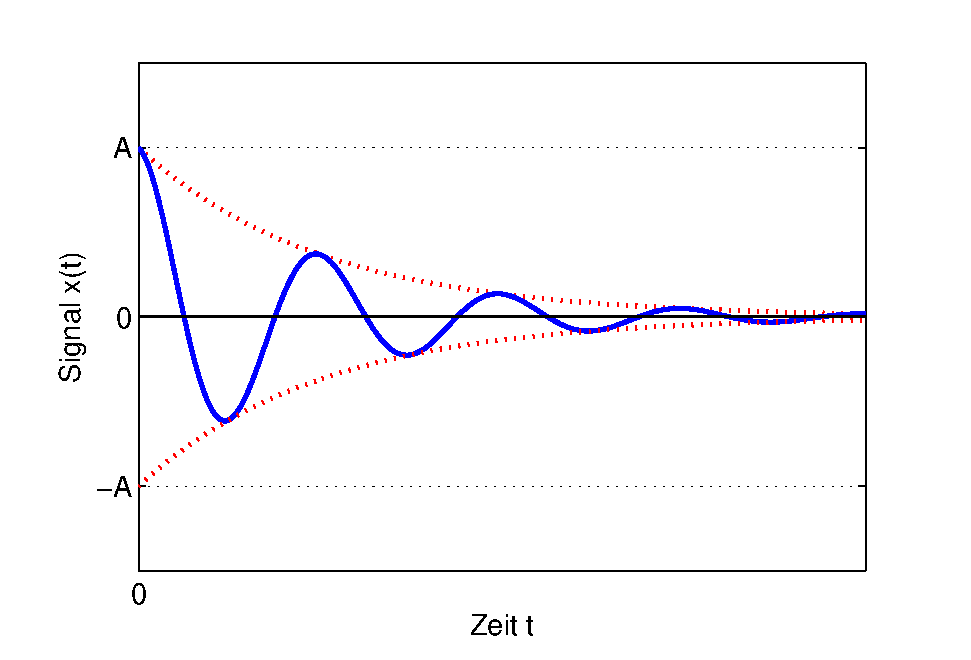
\includegraphics[width=0.5\textwidth]{Kapitel1/Bilder/image25}}
  \caption{Darstellung einer Exponentialfunktion mit abklingender Amplitude}
  \label{fig:KomplexExponentialfunktion}
\end{figure}

\noindent Bild \ref{fig:KomplexExponentialfunktion3D} zeigt eine r\"{a}umliche Darstellung der komplexen Exponentialfunktion und die Projektion der Funktion auf die Realteil-Zeit-Ebene.

\begin{figure}[H]
  \centerline{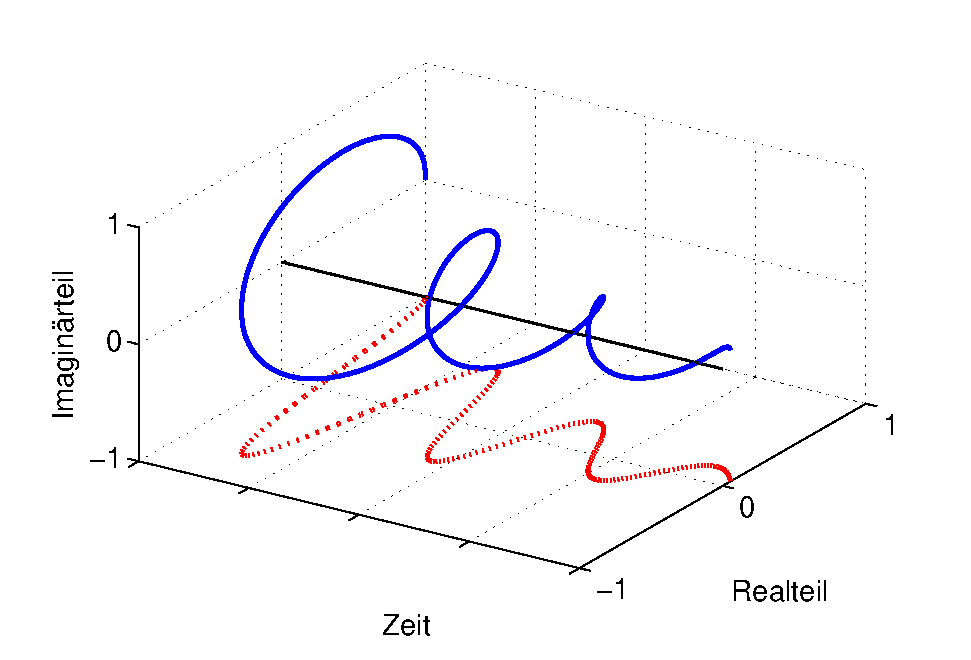
\includegraphics[width=0.5\textwidth]{Kapitel1/Bilder/image26}}
  \caption{R\"{a}umliche Darstellung der komplexen Exponentialfunktion und Projektion der Funktion auf die Realteil-Zeit-Ebene}
  \label{fig:KomplexExponentialfunktion3D}
\end{figure}

\noindent Die Projektion der komplexen Exponentialfunktion auf die Realteil-Zeit-Ebene ergibt die abklingende harmonische Schwingung.

\begin{equation}\label{eq:oneninetyseven}
x\left(t\right)=A\cdot e^{\delta _{0} \cdot t} \cdot \cos \left(\omega _{0} \cdot t\right)\cdot \sigma \left(t\right)
\end{equation}

\noindent Je nach Lage des Wertes $\lambda = \delta{}_{0} + j.\omega{}_{0}$ in der komplexen Ebene, ergibt sich ein charakteristisches Verhalten der komplexen Exponentialfunktion. Bei der Diskussion von Systemeigenschaften linearer Systeme wird die Interpretation reeller und komplexer Exponentialfunktionen weiter vertieft.\newline


\InsertBoxL{0}{
\includegraphics[scale=0.5]{Code.JPG}} 
\textcolor{white}{.}\newline
\noindent Im Online-Portal \textit{Systemtheorie Online} verdeutlicht die Applikation \textit{Komplexe Exponentialfunktion} den Zusammenhang zwischen der Lage des Wertes $\lambda$ = $\delta$ + j$.$$\omega$${}_{0}$ in der komplexen Ebene und dem Verhalten der Schwingung.


\clearpage


\subsubsection{ Zusammenfassung zur Beschreibung von Einschwingvorg\"{a}ngen}

\noindent Die Systemreaktion linearer Systeme ist in vielen Anwendungen eine abklingende harmonische Schwingung. In Tabelle \ref{tab:twofive} werden die wesentlichen Funktionen für die mathematische Beschreibung der Einschwingvorgänge zusammengestellt.

\begin{table}[H]
\setlength{\arrayrulewidth}{.1em}
\caption{Funktionen zur Beschreibung von Einschwingvorgängen}
\setlength{\fboxsep}{0pt}%
\colorbox{lightgray}{%
\arrayrulecolor{white}%
\begin{tabular}{| c | c |}
\hline
\parbox[c][0.28in][c]{3.3in}{\smallskip\centering\textbf{\fontfamily{phv}\selectfont{Funktion}}} & \parbox[c][0.28in][c]{3.3in}{\smallskip\centering\textbf{\fontfamily{phv}\selectfont{Mathematische Beschreibung}}}\\ \hline

\parbox[c][0.64in][c]{3.3in}{\centering{\fontfamily{phv}\selectfont{Periodische Funktion der Periodendauer T}}} &
\parbox[c][0.64in][c]{3.3in}{\centering{$x\left(t\right)=x\left(t+k\cdot T_{0} \right)$}}\\ \hline

\parbox[c][0.64in][c]{3.3in}{\centering{\fontfamily{phv}\selectfont{Harmonische Funktion}}} & 
\parbox[c][0.64in][c]{3.3in}{\centering{$x\left(t\right)=A\cdot \cos \left(\omega _{0} \cdot t+\varphi \right)=A\cdot \cos \left(\omega _{0} \cdot \left(t+t_{0} \right)\right)$}}\\ \hline

\parbox[c][1in][c]{3.3in}{\centering{\fontfamily{phv}\selectfont{Additionstheoreme für harmonische Funktionen}}} & 
\parbox[c][1in][c]{3.3in}{\centering{$\sin \left(a+b\right)=\sin \left(a\right)\cdot \cos \left(b\right)+\cos \left(a\right)\cdot \sin \left(b\right)$$\sin \left(a-b\right)=\sin \left(a\right)\cdot \cos \left(b\right)-\cos \left(a\right)\cdot \sin \left(b\right)$$\cos \left(a+b\right)=\cos \left(a\right)\cdot \cos \left(b\right)-\sin \left(a\right)\cdot \sin \left(b\right)$$\cos \left(a-b\right)=\cos \left(a\right)\cdot \cos \left(b\right)+\sin \left(a\right)\cdot \sin \left(b\right)$}}\\ \hline

\parbox[c][0.64in][c]{3.3in}{\centering{\fontfamily{phv}\selectfont{Eulersche Darstellung}}} & 
\parbox[c][0.64in][c]{3.3in}{\centering{$e^{j\cdot \varphi } =\cos \left(\varphi \right)+j\cdot \sin \left(\varphi \right)$}}\\ \hline

\parbox[c][0.64in][c]{3.3in}{\centering{\fontfamily{phv}\selectfont{Darstellung der Kosinusfunktion über die Eulersche Formel}}} &
\parbox[c][0.64in][c]{3.3in}{\centering{$\cos \left(\varphi \right)=\dfrac{1}{2} \cdot \left(e^{j\cdot \varphi } +e^{-j\cdot \varphi } \right)$}}\\ \hline

\parbox[c][0.64in][c]{3.3in}{\centering{\fontfamily{phv}\selectfont{Darstellung der Sinusfunktion über die Eulersche Formel}}} &
\parbox[c][0.64in][c]{3.3in}{\centering{$e^{j\cdot \varphi } =\cos \left(\varphi \right)+j\cdot \sin \left(\varphi \right)$}}\\ \hline

\parbox[c][0.64in][c]{3.3in}{\centering{\fontfamily{phv}\selectfont{Exponentialfunktion mit komplexem Argument}}} & 
\parbox[c][0.64in][c]{3.3in}{\centering{$e^{\lambda \cdot t} =e^{\left(\delta _{0} +j\cdot \omega _{0} \right)\cdot t} =e^{\delta _{0} \cdot t} \cdot e^{j\cdot \omega _{0} \cdot t} $}}\\ \hline

\parbox[c][1.4in][c]{3.3in}{\centering{\fontfamily{phv}\selectfont{Beschreibung einer gedämpften Schwingung über eine Exponentialfunktion mit komplexem Argument}}} &
\parbox[c][1.4in][c]{3.3in}{\centering{$\begin{array}{rcl} {x(t)} & {=} & {A\cdot e^{\delta _{0} \cdot t} \cdot \cos \left(\omega _{0} \cdot t\right)\cdot \sigma \left(t\right)} \\  
\\
{} & {=} & {\dfrac{1}{2} \cdot A\cdot e^{\delta _{0} \cdot t} \cdot \left(e^{j\cdot \omega _{0} \cdot t} +e^{-j\cdot \omega _{0} \cdot t} \right)\cdot \sigma \left(t\right)} \\
\\
{} & {=} & {\dfrac{1}{2} \cdot A\cdot \left(e^{\left(\delta _{0} +j\cdot \omega _{0} \right)\cdot t} +e^{\left(\delta _{0} -j\cdot \omega _{0} \right)\cdot t} \right)\cdot \sigma \left(t\right)} \end{array}$}}\\ \hline


\end{tabular}%
}
\label{tab:twofive}
\end{table}


\clearpage

\subsection{ Normierung von Signalen}

\noindent In den Beispielen der vorangegangenen Abschnitte sind die Einheiten der Signale mitgef\"{u}hrt. Das hat den Vorteil, dass durch eine Umrechnung der Einheiten eine Konsistenzpr\"{u}fung durchgef\"{u}hrt werden kann. In komplexeren Anwendungen und Beispielen steigt der Aufwand f\"{u}r das Mitf\"{u}hren von Einheiten aber schnell an. Durch eine Normierung der physikalischen Gr\"{o}{\ss}en lassen sich die Ausdr\"{u}cke oft stark vereinfachen. Dieser Vorteil wird jedoch durch die nicht mehr m\"{o}gliche Plausibilisierung der Rechenergebnisse anhand von Einheiten erkauft. Als Hintergrundinformation f\"{u}r das Rechnen ohne Einheiten wird die Methode der Normierung von Signalen vorgestellt. Sie teilt sich in zwei Schritte auf:

\bigskip

{\fontfamily{phv}\selectfont
\noindent\textbf{Amplitudennormierung}} \smallskip

\noindent Bei der Amplitudennormierung werden alle Signale als dimensionsloses Vielfaches einer Bezugsgrö{\ss}e ausgedrückt. Die einfachste Art der Normierung ist der Bezug der jeweiligen Grö{\ss}e auf die SI-Einheit. Wegen der Kohärenz des SI-Einheitensystems bleibt bei dieser Art der Normierung der Zahlenwert aller Grö{\ss}en gleich. Die Normierung physikalischer Grö{\ss}en mit den jeweiligen SI-Einheiten ist einfach, die dabei entstehenden Grö{\ss}en sind jedoch oft unhandlich. 

\bigskip

{\fontfamily{phv}\selectfont
\noindent\textbf{Zeitnormierung}} \smallskip

\noindent Eine Zeitnormierung bedeutet, dass alle Zeitangaben als dimensionsloses Vielfaches einer Bezugszeit ausgedr\"{u}ckt werden. Insbesondere bei Systemen, die in festen Zeitintervallen abgetastet werden, bietet sich eine Zeitnormierung mit dieser Abtastzeit an. 

\noindent Die Amplituden- und Zeitnormierung von Signalen hat auch Konsequenzen f\"{u}r die Bauelemente, was im Folgenden f\"{u}r elektrische Systeme hergeleitet wird. Der Index N wird bei dieser Darstellung f\"{u}r normierte Gr\"{o}{\ss}e verwendet. Eine Amplitudennormierung mit der Spannung U${}_{0}$ beziehungsweise dem Strom I${}_{0}$ f\"{u}hrt zu einer normierten Spannung U${}_{N}$ 


\begin{equation}\label{eq:oneninetyeight}
U_{N} =\dfrac{U}{U_{0} }
\end{equation}

\noindent beziehungsweise einem normierten Strom I${}_{N}$

\begin{equation}\label{eq:oneninetynine}
I_{N} =\dfrac{I}{I_{0} }
\end{equation}


\noindent Eine Zeitnormierung normiert die Zeit t auf eine Bezugszeit T${}_{0}$, und es ergibt sich eine normierte Zeit t${}_{N}$

\begin{equation}\label{eq:onehundred}
t_{N} =\dfrac{t}{T_{0} }
\end{equation}


\noindent Mit der Normierung der Zeit geht auch eine Normierung der Frequenz einher. Die normierte Frequenz f${}_{N}$ berechnet sich aus

\begin{equation}\label{eq:onehundredone}
f_{N} =\dfrac{{\rm 1}}{{\rm t}_{{\rm N}} } {\rm \; }=\dfrac{{\rm T}_{{\rm 0}} }{{\rm t}} =f\cdot T_{0}
\end{equation}


\noindent Aus der Normierung von Amplituden und Zeit ergibt sich eine Normierung der Bauelemente. Unmittelbar deutlich wird das an dem ohmschen Widerstand R.

\begin{equation}\label{eq:onehundredtwo}
R=\dfrac{{\rm U}}{I} {\rm \; }=\dfrac{{\rm U}_{{\rm N}} \cdot {\rm U}_{{\rm 0}} }{I_{N} \cdot I_{0} } =R_{N} \cdot R_{0}
\end{equation}


\noindent Ein normierter ohmscher Widerstand R${}_{N}$ berechnet sich damit aus 

\begin{equation}\label{eq:onehundredthree}
R_{N} =\dfrac{R}{R_{0} } {\rm \; }={\rm R}\cdot \dfrac{{\rm I}_{{\rm 0}} }{U_{0} }
\end{equation}


\noindent In einer vergleichbaren Weise k\"{o}nnte hergeleitet werden, was die Normierung f\"{u}r Induktivit\"{a}t und Kapazit\"{a}t bedeutet. Besonders anschaulich wird dies bei der Umrechnung von Zeitkonstanten eines RC-Glieds.

\begin{equation}\label{eq:onehundredfour}
T=R\cdot C
\end{equation}


\noindent Die Kapazit\"{a}t C berechnet sich durch Umstellen der Gleichung zu 

\begin{equation}\label{eq:onehundredfive}
C=\dfrac{T}{R} {\rm \; }=\dfrac{T_{N} \cdot T_{0} }{R_{N} \cdot R_{0} } =C_{N} \cdot C_{0}
\end{equation}

\noindent Die normierte Kapazit\"{a}t C${}_{N}$ betr\"{a}gt damit

\begin{equation}\label{eq:onehundredsix}
C_{N} =\dfrac{C}{C_{0} } \; =C\cdot \dfrac{R_{0} }{T_{0} }
\end{equation}

\noindent Eine vergleichbare Herleitung f\"{u}hrt zu der normierten Induktivit\"{a}t 

\begin{equation}\label{eq:onehundredseven}
L_{N} =\dfrac{L}{L_{0} } \; =L\cdot \dfrac{1}{R_{0} \cdot T_{0} } 
\end{equation}

\noindent
\colorbox{lightgray}{%
\arrayrulecolor{white}%
\renewcommand\arraystretch{0.6}%
\begin{tabular}{ wl{16.5cm} }
{\fontfamily{phv}\selectfont
\noindent{Beispiel: Normierung RC-Glied}}
\end{tabular}%
}\bigskip


\noindent Die Normierung von Gr\"{o}{\ss}en soll anhand des RC-Netzwerks aus Bild \ref{fig:RCNETZWERK} durchgef\"{u}hrt werden. 

\noindent 

\begin{figure}[ht]
  \centerline{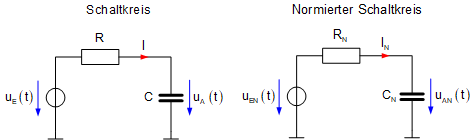
\includegraphics[width=0.7\textwidth]{Kapitel1/Bilder/image27}}
  \caption{Beispiel RC-Netzwerk, normierte und nicht normierte Darstellung }
  \label{fig:RCNETZWERK}
\end{figure}



\noindent Die Kapazit\"{a}t hat einen Wert von C = 1 µF und der Widerstand betr\"{a}gt R = 1 k$\Omega$. Das System wird normiert mit den Gr\"{o}{\ss}en
\begin{equation}\label{eq:onehundredeight}
U_{0} =1  \; V
\end{equation}

\begin{equation}\label{eq:onehundrednine}
{I}_{0} \; =1 \;mA
\end{equation}

\begin{equation}\label{eq:onehundredten}
{t}_{0} =1 \; ms
\end{equation}


\noindent Die normierten Bauelemente haben damit die Werte

\begin{equation}\label{eq:onehundredeleven}
R_{N} =\dfrac{R\cdot I_{0} }{U_{0} } =\dfrac{1{\rm \; }k\Omega \cdot 1{\rm \; }mA}{1V} =1
\end{equation}

\noindent und 

\begin{equation}\label{eq:onehundredtwelve}
C_{N} =C\cdot \dfrac{R_{0} }{T_{0} } =1 \; \mu F\cdot \dfrac{1 \; k\Omega }{1 \; ms} =1
\end{equation}


\noindent Das Ersatzschaltbild des normierten Systems ist in Bild \ref{fig:RCNETZWERK} rechts dargestellt.

\bigskip

{\fontfamily{phv}\selectfont
\noindent\textbf{Zusammenfassung Normierung von Signalen}} \smallskip

\noindent Im Folgenden werden Beispiele normiert berechnet, um die Darstellung kompakter zu halten. Nur in Einzelfällen werden die Einheiten zur Herleitung von Zeitkonstanten, Grenzfrequenzen oder anderen charakteristischen Größen mitgeführt. Die Schritte zur Normierung von Signalen sind in Tabelle \ref{tab:twosix} zusammengefasst.

{\fontfamily{phv}\selectfont
\noindent\textbf{}} \smallskip

\medskip
\begin{table}[H]
\setlength{\arrayrulewidth}{.1em}
\caption{Schritte zur Normierung von Signalen}
\setlength{\fboxsep}{0pt}%
\colorbox{lightgray}{%
\arrayrulecolor{white}%
\begin{tabular}{| c | c |}
\hline
\parbox[c][0.28in][c]{3.3in}{\smallskip\centering\textbf{\fontfamily{phv}\selectfont{Normierung}}} & \parbox[c][0.28in][c]{3.3in}{\smallskip\centering\textbf{\fontfamily{phv}\selectfont{Mathematische Beschreibung}}}\\ \hline

\parbox[c][0.64in][c]{3.3in}{\centering{\fontfamily{phv}\selectfont{Amplitudennormierung}}} & 
\parbox[c][0.64in][c]{3.3in}{\centering{$U_{N} =\dfrac{U}{U_{0} } $}}\\ \hline

\parbox[c][0.64in][c]{3.3in}{\centering{\fontfamily{phv}\selectfont{Zeitnormierung}}} & \parbox[c][0.64in][c]{3.3in}{\centering{$t_{N} =\dfrac{t}{T_{0} } $}}\\
\end{tabular}%
}
\label{tab:twosix}
\end{table}

\bigskip

\noindent In der Regelungstechnik wird statt der hier dargestellten Normierung von Signalen eine Skalierung vorgenommen. Bei der Skalierung werden die Amplituden der Signale geeignet normiert, eine Zeitnormierung findet nicht statt.

\clearpage



\subsection{ Literatur}


\subsubsection{ Literaturstellen zur mathematischen Darstellung}

\begin{tabular}{|p{0.6in}|p{5.7in}|} \hline 
[Papu11] & Papula, Lothar: Mathematik f\"{u}r Ingenieure und Naturwissenschaftler Band 1 - 3, Springer Fachmedien Wiesbaden, 2011 \\ \hline 
[Bron79] & Bronstein, Ilja: Taschenbuch der Mathematik, Wissenschaftlicher Verlag Harri Deutsch, Frankfurt am Main, 2008 \\ \hline 
\end{tabular}


\subsubsection{ Weiterf\"{u}hrende Literatur}

\begin{tabular}{|p{0.6in}|p{5.7in}|} \hline 
[Saue12] & R. Sauer, I. Szabo (Hrsg.): Mathematische Hilfsmittel des IngenieursSpringer-Verlag, 2012 \\ \hline 
[Gelf67] & Gelfand, Israel: Verallgemeinerte Funktionen (Distributionen): Verallgemeinerte Funktionen und das Rechnen mit IhnenVEB Deutscher Verlag der Wissenschaften, Berlin (Ost), 1967. \\ \hline 
[Foel11] & F\"{o}llinger, Otto: Laplace-, Fourier- und z-Transformation. 10., \"{u}berarbeitete AuflageVDE Verlag GmbH, Berlin, Offenbach 2011 \\ \hline 
[Giro05] & Girod, Bernd: Einf\"{u}hrung in die Systemtheorie. 3. AuflageB.G. Teubner Stuttgart, 2005 \\ \hline 
\end{tabular}